\begin{flushright}
\textbf{Solutions prepared by Prajwala TM $<$prajwala.tm@gmail.com$>$}
\end{flushright}
\section*{Exercises}
\vskip 1cm

\setcounter{Exercise}{0}
\setcounter{Answer}{0}


\section*{Transistors and Logic Gates}

\begin{ExerciseList}
\Exercise
Describe the operation of a P-N junction.
\Answer
The majority carriers on the $n$ side are electrons whereas those on the $p$ side are holes. When a junction is formed in a silicon wafer by doping, a concentration gradient is created between $p$-type and $n$-type materials. This results in electrons moving from $n$ side to 
$p$ side and holes moving from $p$ side to $n$ side through the junction. When an electron leaves the $n$-side region, it leaves behind an ionised donor (a positive charge). Similarly when a hole is diffused to $n$-side, it leaves behind an ionised acceptor (a negative charge).  This movement of electrons from $n$-side to $p$-side (n$\rightarrow$p) and the movement of holes from $p$-side to $n$-side is called (p$\rightarrow$n) “diffusion” and it results in a current named as “diffusion current“.When more and more electrons leaves the $n$-region and more and more holes leaves the $p$-region, a region of positive and negative charges is formed at the junction. Positive charges get accumulated near the $n$-side junction and negative charges get accumulated near the $p$-side junction. This region is known as “depletion” region.Thus, there is a layer of -ve charges accumulated at the $p$-side of junction and a layer of +ve charges accumulated at the $n$-side of the junction. This results in the formation of an electric field directed from positive charge to negative charge. This electric field causes electrons to move from $p$ side to $n$ side (p$\rightarrow$n) and the holes to move from $n$ side to $p$ side 
(n$\rightarrow$p). This motion of charge carriers due to electric field is known as “drift”.The current resulting from the flow of electrons and holes due to this electric field (generated by depletion region) is known as “drift current”.
At steady state, the drift and diffusion currents balance each other , and there is effectively "NO CURRENT FLOW" across the junction.
\Exercise
Define drift and diffusion current.
\Answer
Diffusion current is the current in a p-n junction caused by the diffusion of charge carriers (holes and/or electrons) due to the concentration gradient between the n and p sides of the p-n junction. The drift current is the current due to the motion of charge carriers caused by the force exerted on them by an electric field across the depletion region.
\Exercise
Describe the operation of a NMOS transistor? 
\Answer
An NMOS transistor is made by connecting two p-n junctions. It consists of a central substrate of $p$-type doped silicon. There are two small regions on both sides containing $n$-type doped silicon. These are known as $source$ and $drain$ respectively. The region in the middle of the source and drain is known as $channel$. On top of the channel, there is a thin insulating layer typically made of silicon dioxide, and is covered by a metallic or polysilicon based conducting layer. This is called the $gate$.\\
Each of these terminals - source, drain, gate can be connected to a voltage source. The gate voltage can be either logical 1 or logical 0. If the gate voltage is logical 1, then the electrons in the channel get attracted towards the gate. If the voltage at the gate is larger than a certain voltage known as "Threshold voltage", then a low resistance conducting path is formed between the drain and source due to accumulation of electrons. Thus, a current can flow between the drain and source. Hence, when the gate voltage is a logical 1, the NMOS transistor switch is turned on. If its a logical 0, then the switch is turned off. 
\begin{figure}[H]
  \centering
  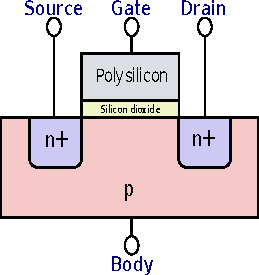
\includegraphics[width=10cm,height=5cm,clip=true,keepaspectratio]{nmos.pdf}
\end{figure}
\Exercise
Draw the circuit of a CMOS inverter, NOR gate, and NAND gate.
\begin{figure}[H]
  \centering
  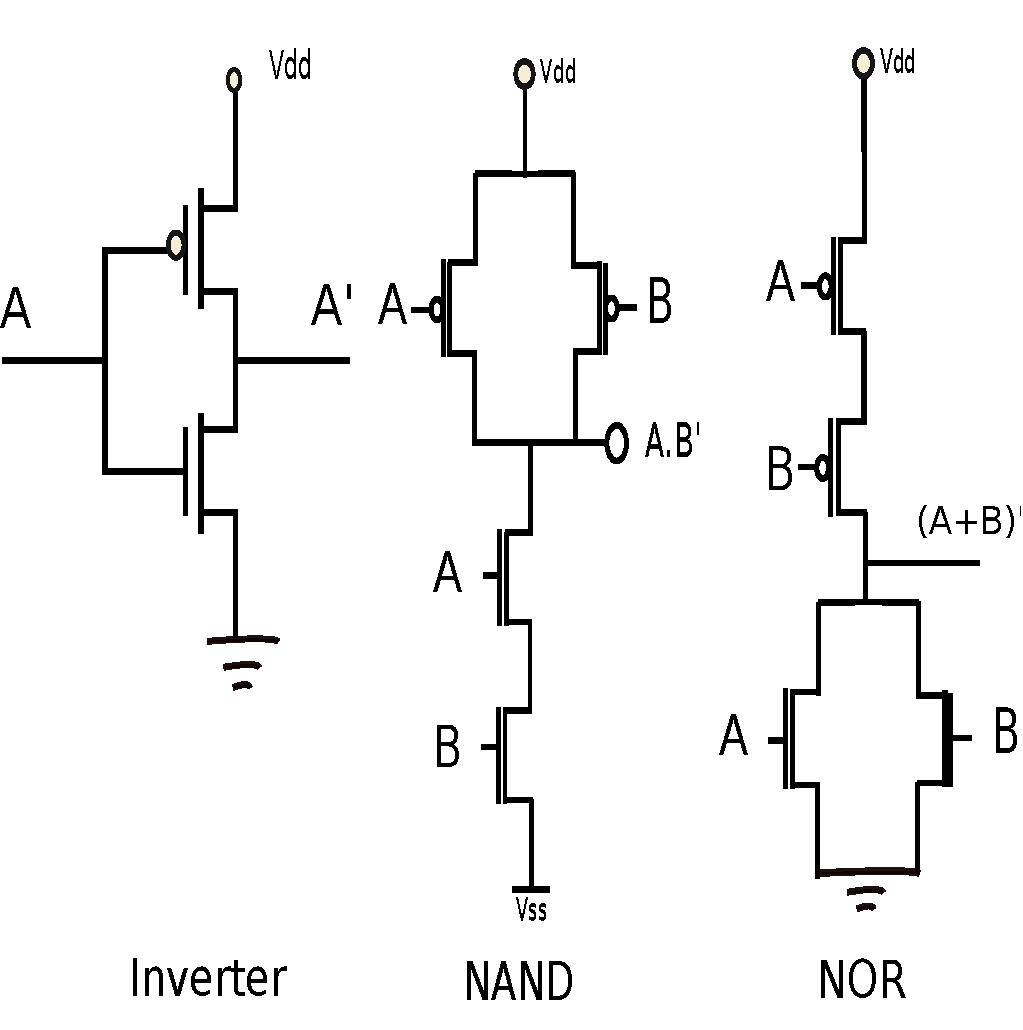
\includegraphics[width=10cm,height=8cm,keepaspectratio]{4.pdf}
\end{figure}
\Exercise
Implement the AND, OR and NOT gates using NAND gates only.
\begin{figure}[H]
  \centering
  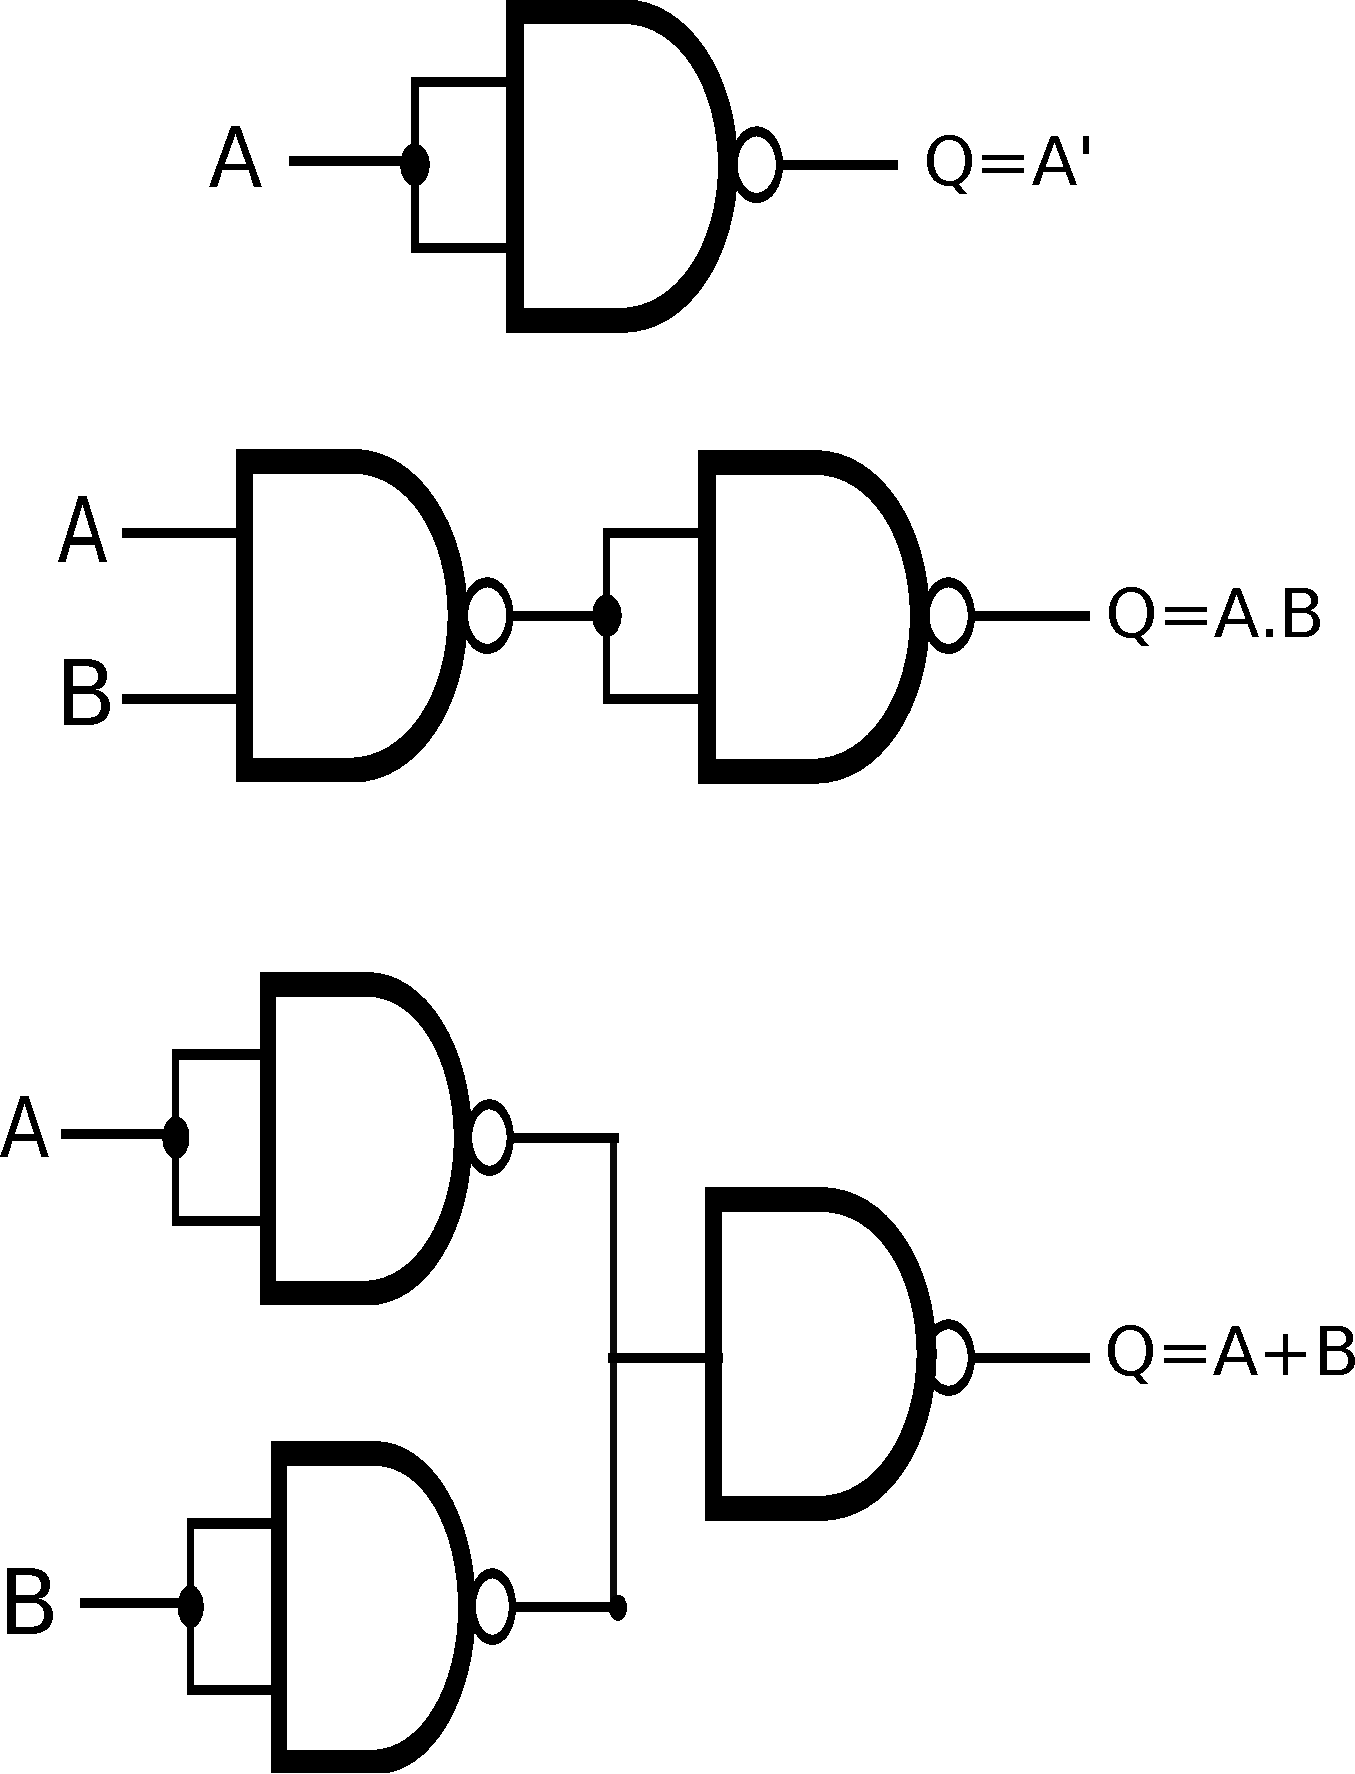
\includegraphics[width=10cm,height=8cm,keepaspectratio]{5.pdf}
\end{figure}
\Exercise
Implement the AND, OR and NOT gates using NOR gates only.
\begin{figure}[H]
  \centering
  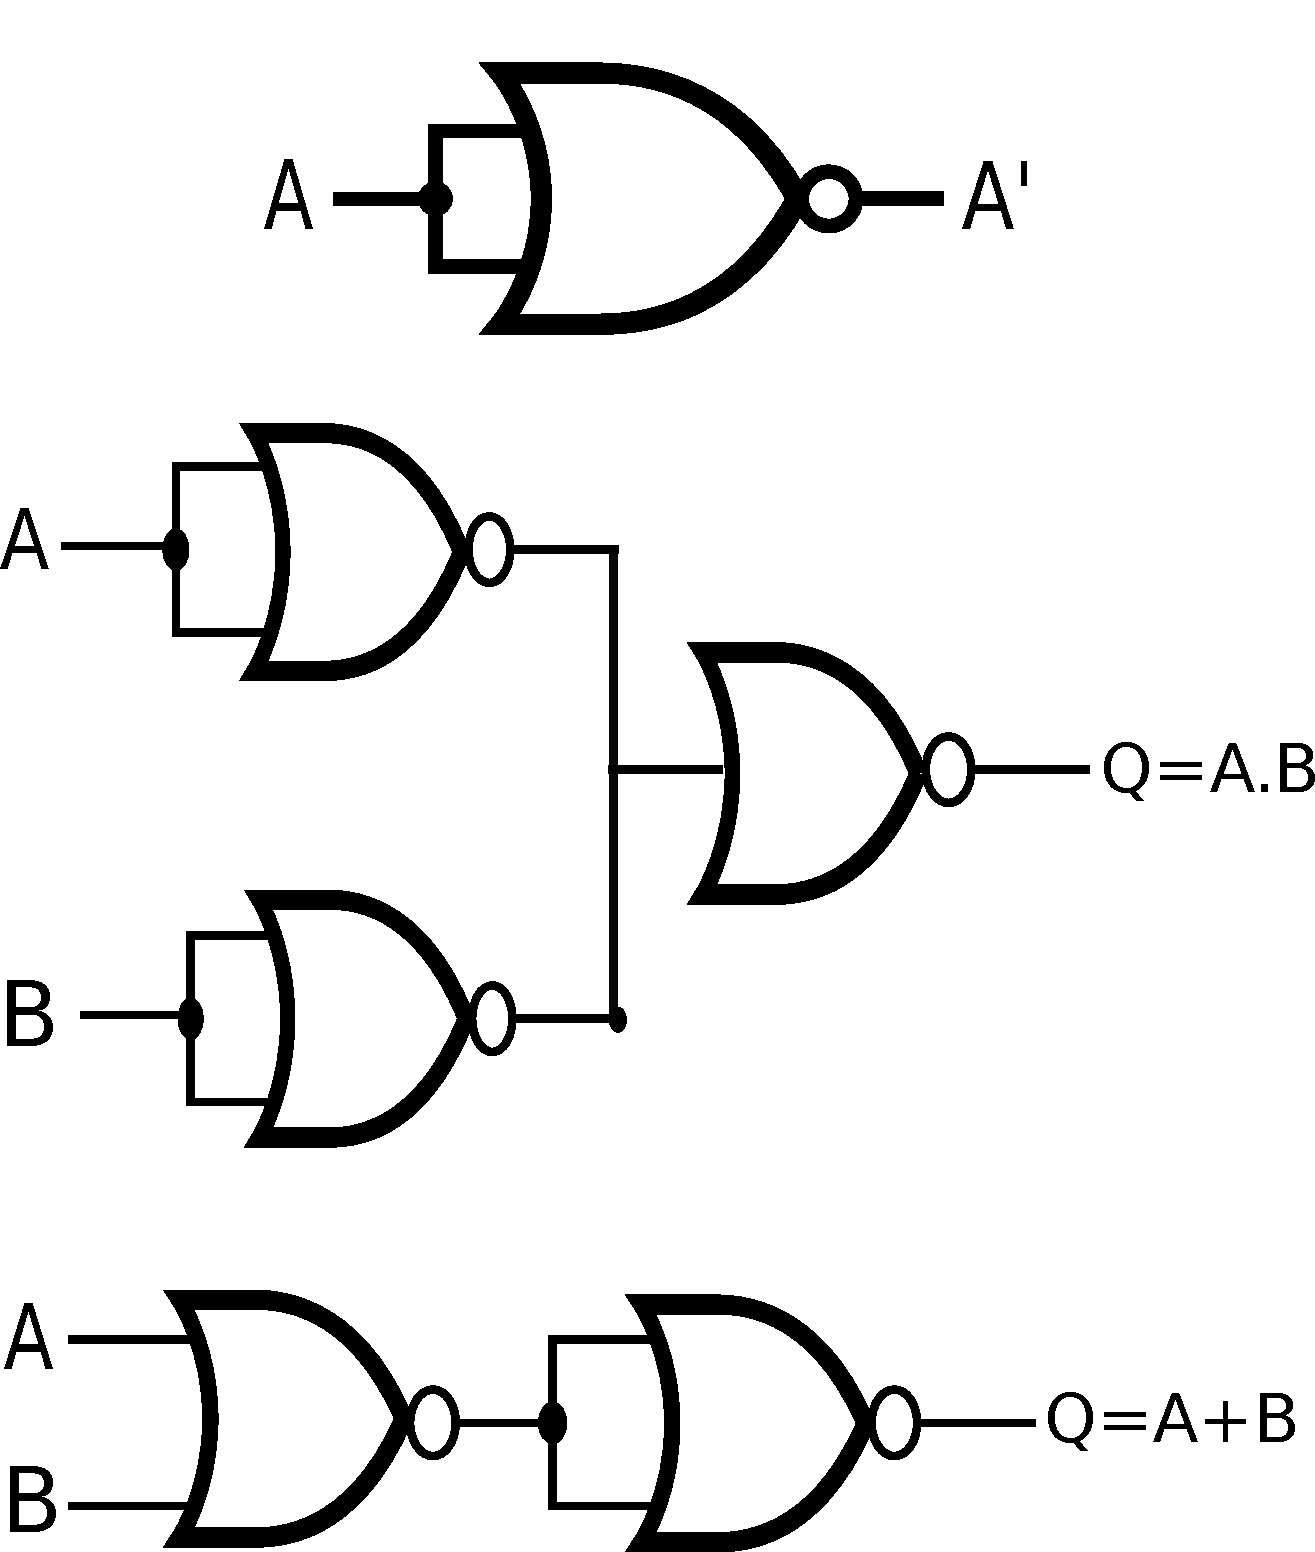
\includegraphics[width=10cm,height=8cm,keepaspectratio]{6.pdf}
\end{figure}
\Exercise
Implement XOR and XNOR gates using NAND gates only.
\begin{figure} [H]
  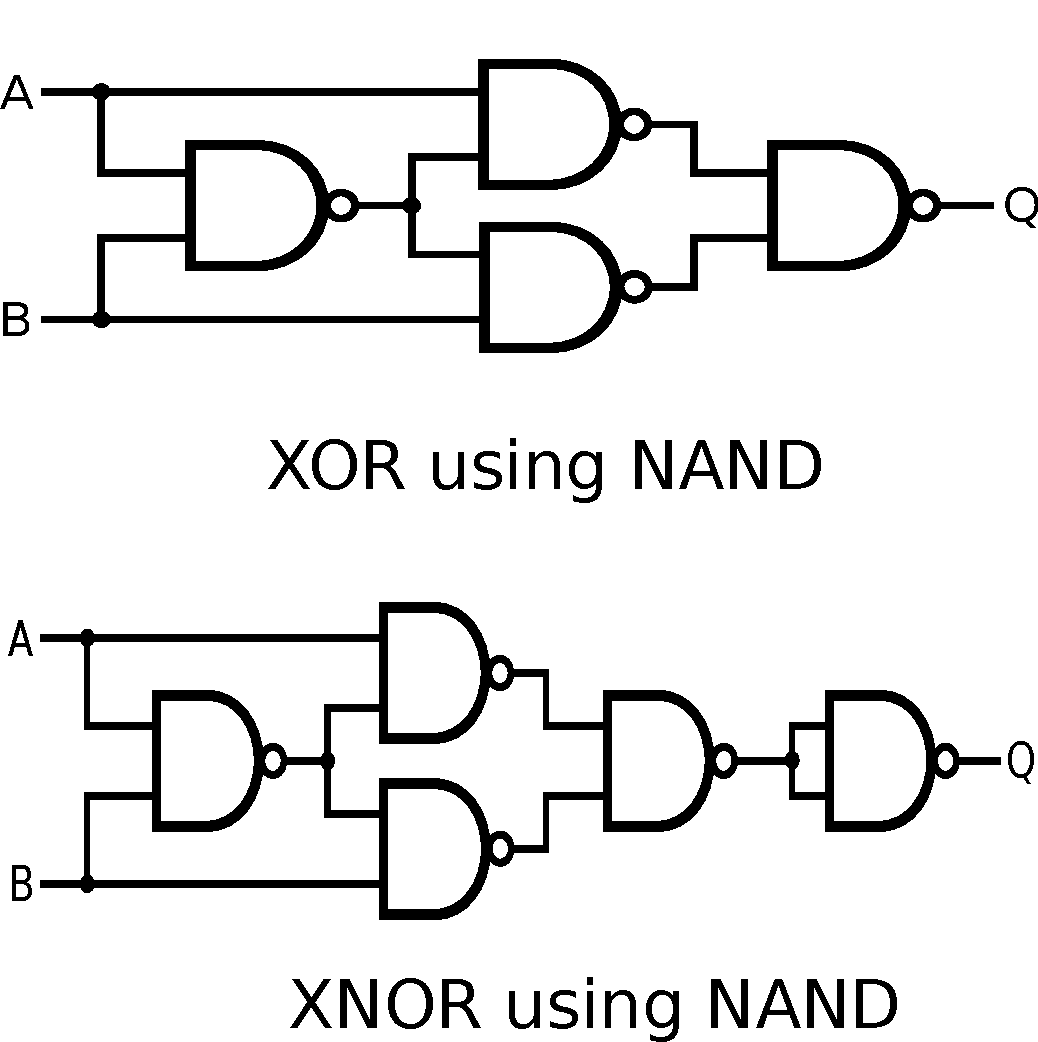
\includegraphics[width=10cm,height=8cm,keepaspectratio]{7xor.pdf}
\end{figure}

\Exercise
\label{que:gatec}
Implement the following Boolean functions by using only AND, OR and NOT gates.
\begin{enumerate}[ a) ]
\item
$\overline A .B + A.\overline B + \overline A.\overline B.\overline C$
\item
$\overline{(A+B+C)}.(\overline A.\overline B+C)$
\item
$\overline{(A+B)}.\overline{(\overline C+\overline D)}$
\item
$\overline A.\overline B.\overline C + A.B.C + \overline D$
\end{enumerate}
a)
\begin{figure} [H]
  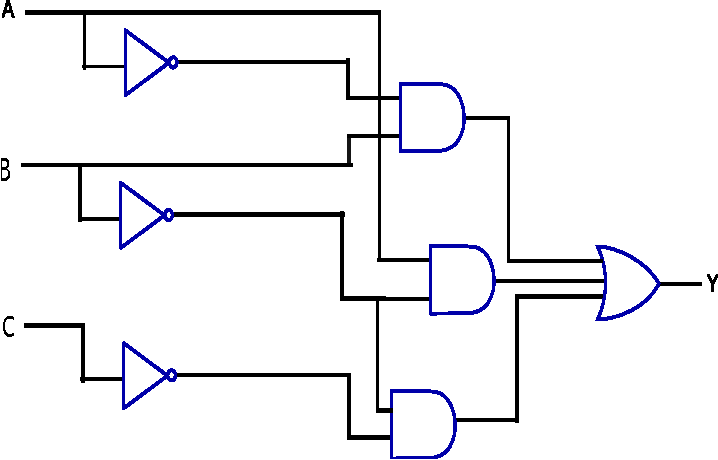
\includegraphics[width=10cm,height=8cm,keepaspectratio]{8a.pdf}
\end{figure}
b)\begin{figure} [H]
  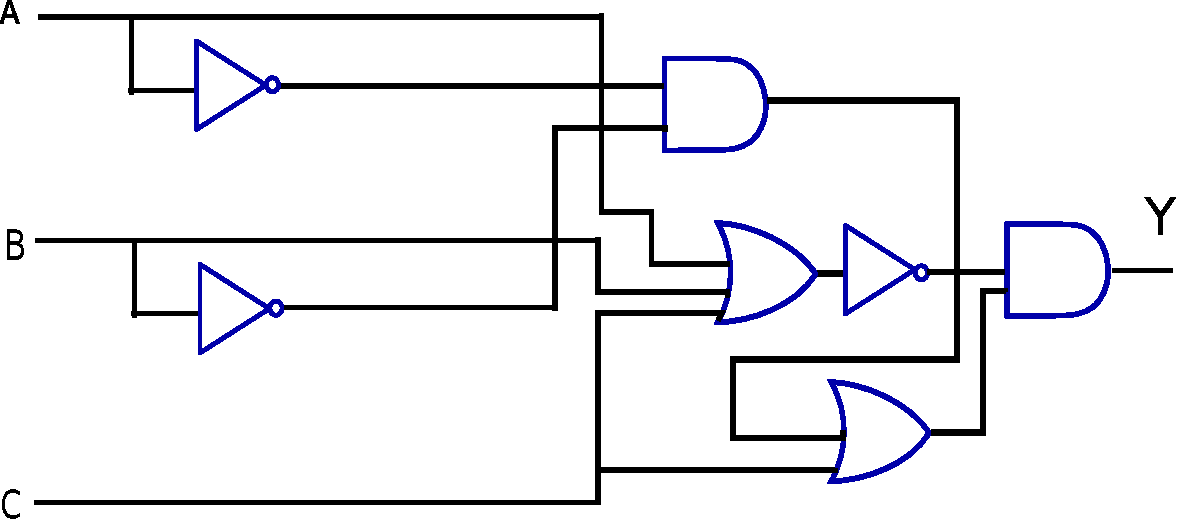
\includegraphics[width=10cm,height=8cm,keepaspectratio]{8b.pdf}
\end{figure}
c)\begin{figure} [H]
  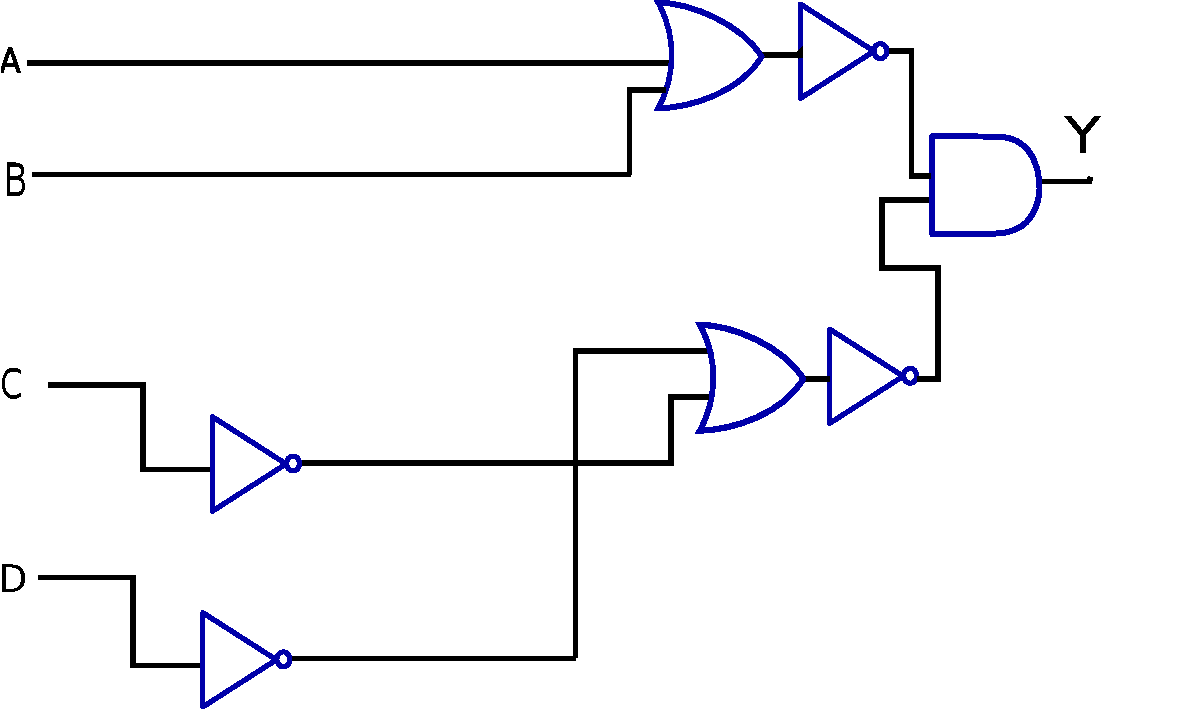
\includegraphics[width=10cm,height=8cm,keepaspectratio]{8c.pdf}
\end{figure}
d)\begin{figure} [H]
  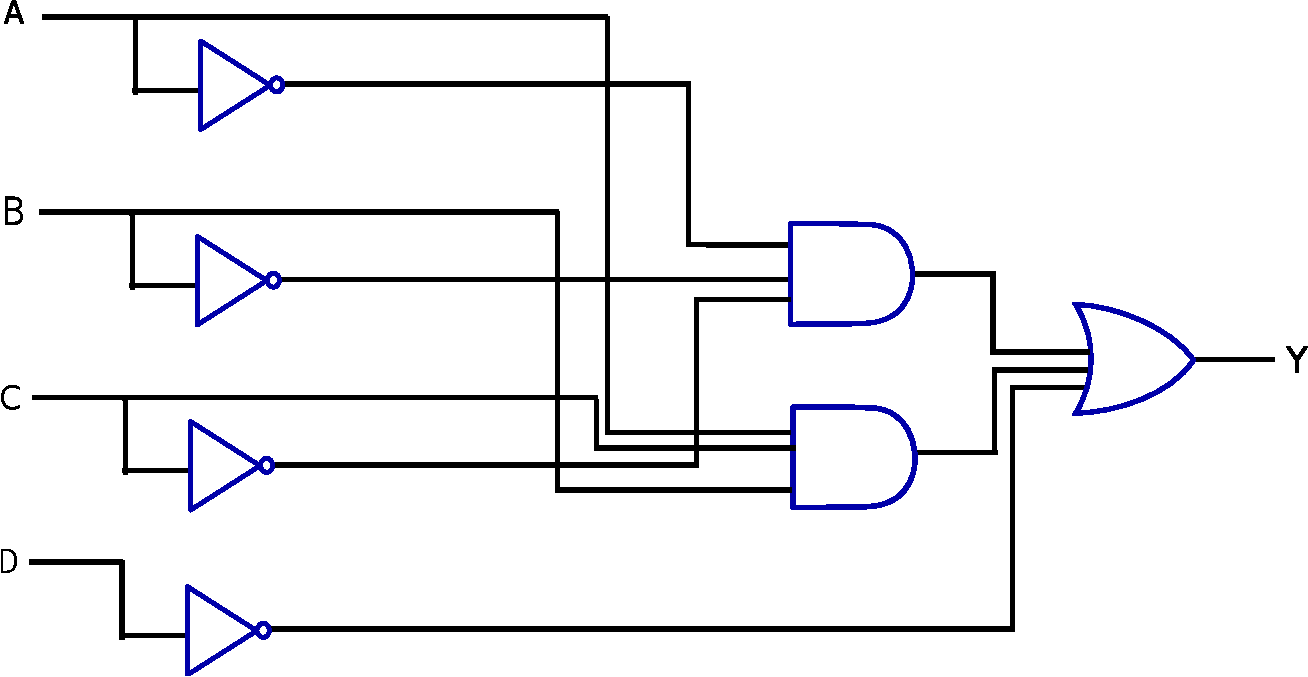
\includegraphics[width=10cm,height=8cm,keepaspectratio]{8d.pdf}
\end{figure}

\Exercise
Answer Question~\ref{que:gatec} by using only NAND gates.

\Answer
a)
\begin{figure} [H]
  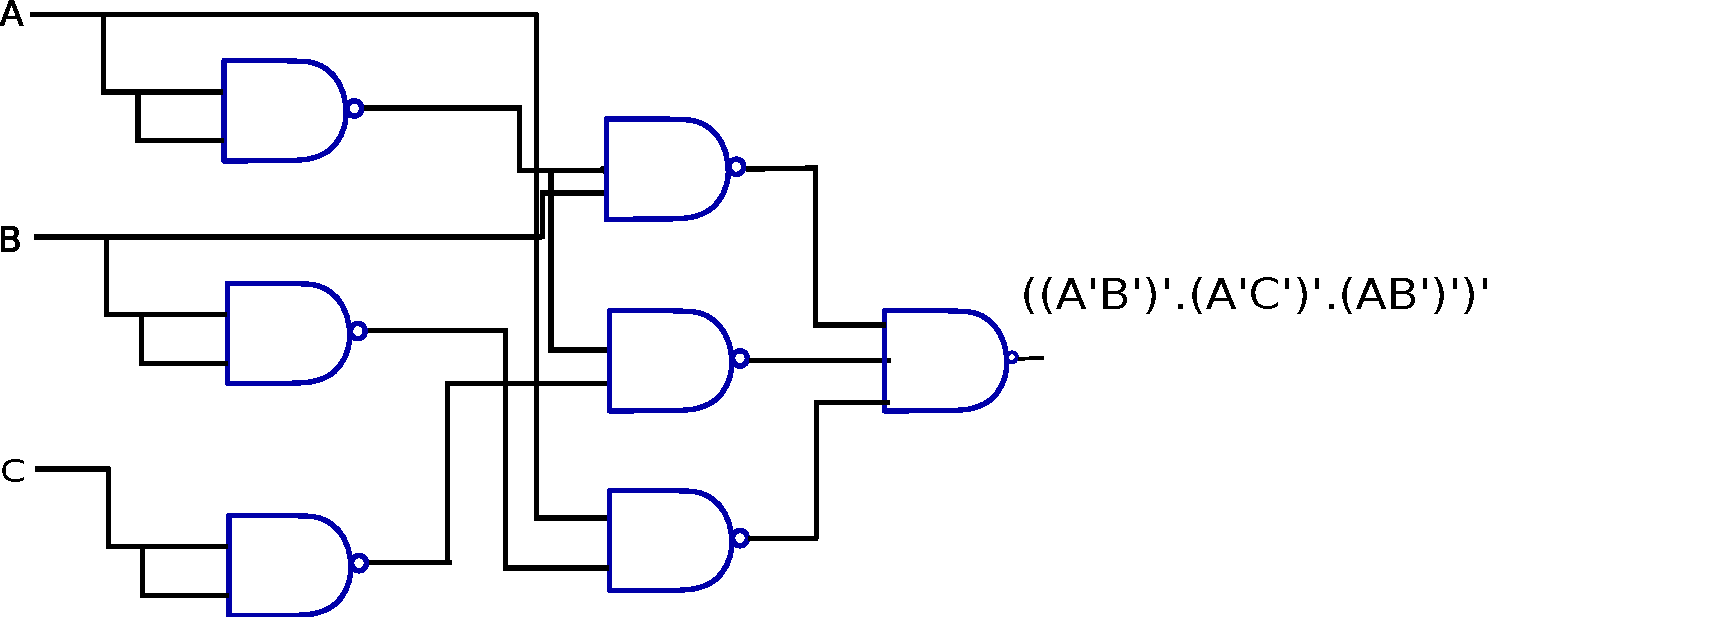
\includegraphics[width=10cm,height=8cm,keepaspectratio]{9a.pdf}
\end{figure}
b)\begin{figure} [H]
  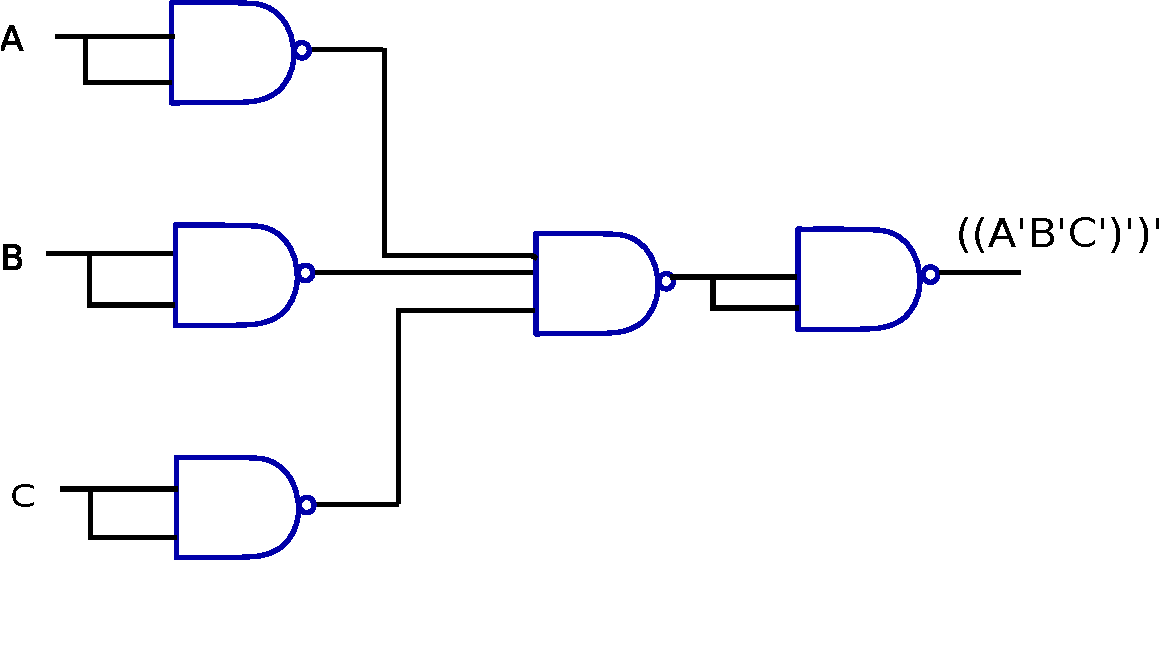
\includegraphics[width=10cm,height=8cm,keepaspectratio]{9b.pdf}
\end{figure}
c)\begin{figure} [H]
  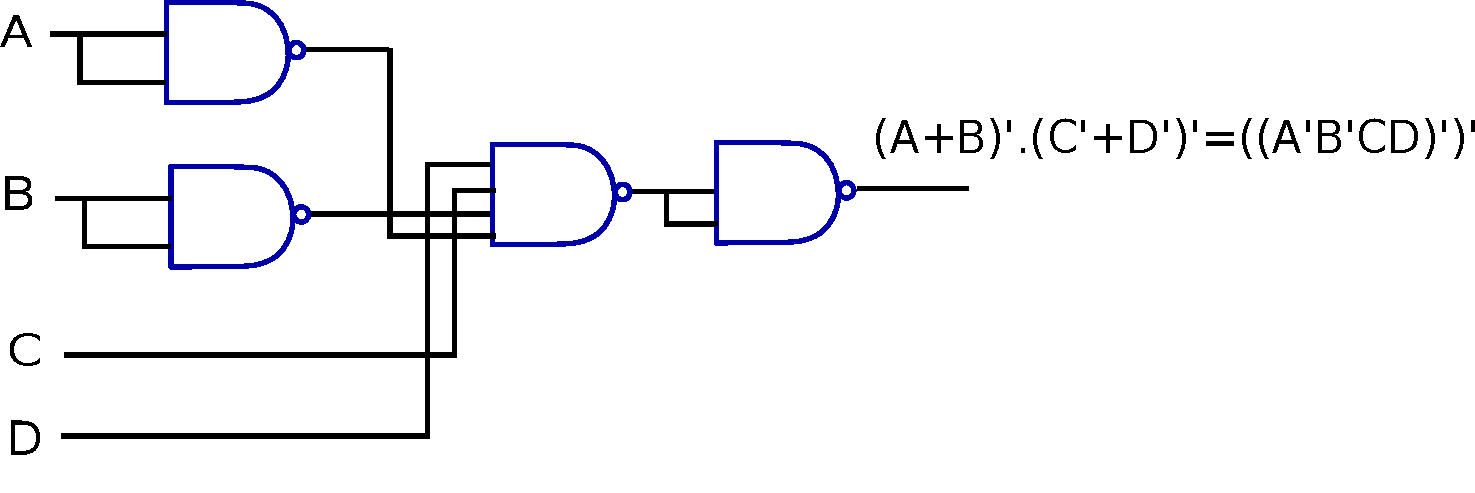
\includegraphics[width=10cm,height=8cm,keepaspectratio]{9c.pdf}
\end{figure}
d)\begin{figure} [H]
  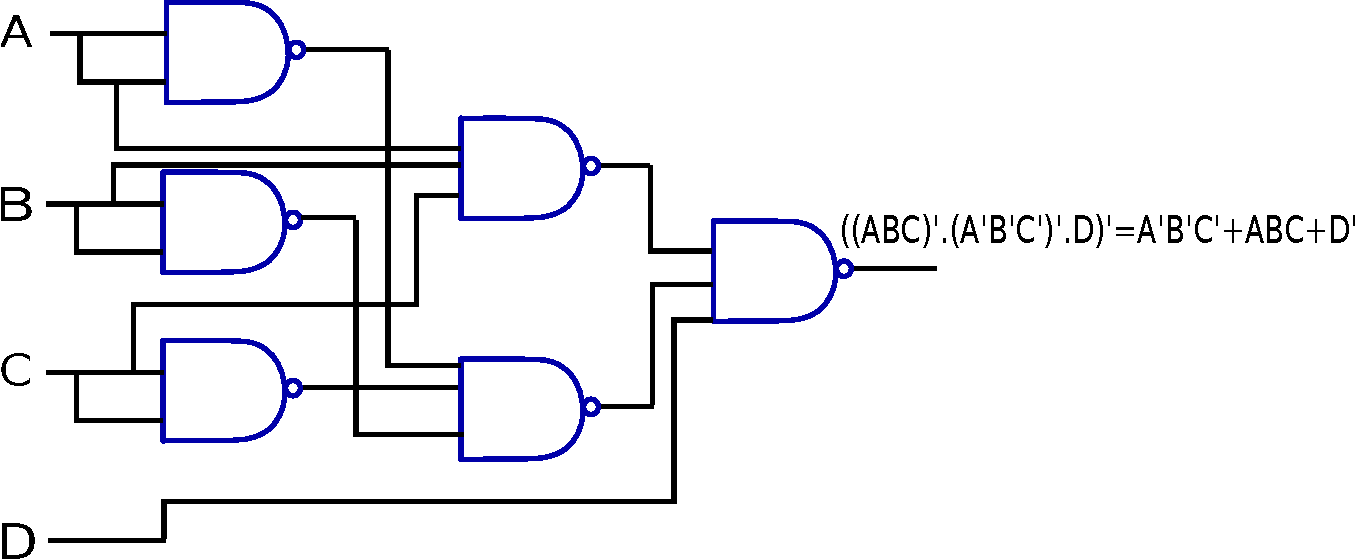
\includegraphics[width=10cm,height=8cm,keepaspectratio]{9d.pdf}
\end{figure}

\end{ExerciseList}

\subsection*{Combinational Logic and Sequential Logic}

\begin{ExerciseList}
\Exercise
Draw the circuit diagram of a $3 \times 8$  decoder.

\begin{figure} [H]
  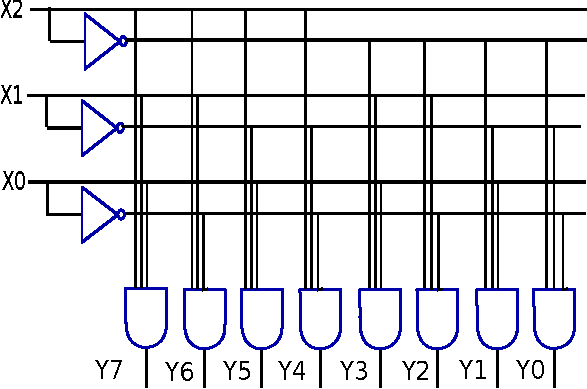
\includegraphics[width=10cm,height=8cm,keepaspectratio]{10.pdf}
\end{figure}
\Exercise
Draw the circuit diagram of a $8-3$ bit encoder.

\begin{figure} [H]
  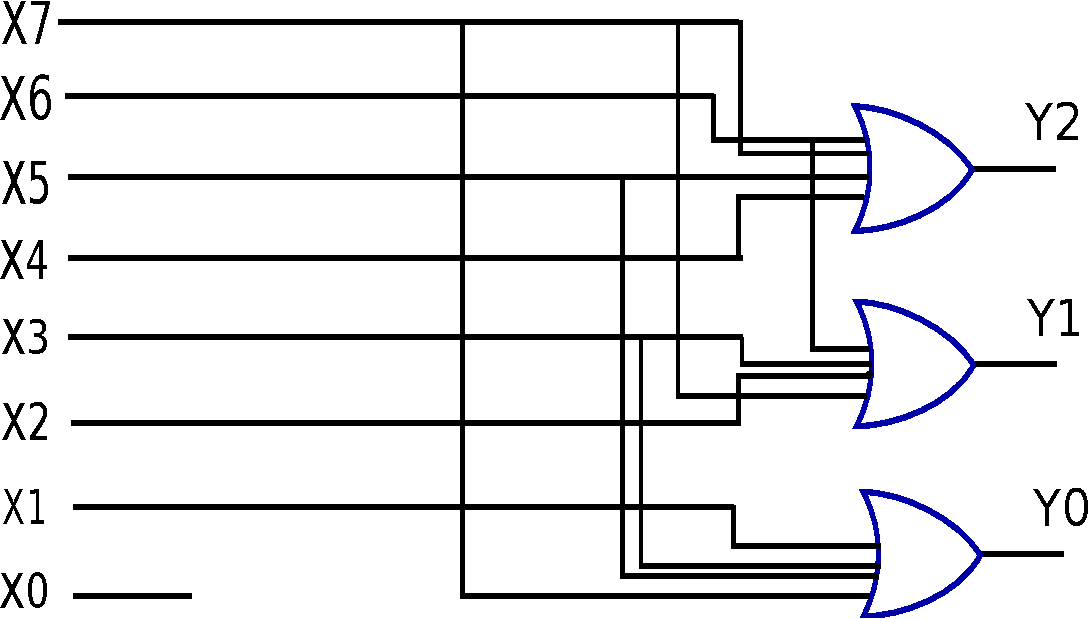
\includegraphics[width=10cm,height=8cm,keepaspectratio]{11.pdf}
\end{figure}

\Exercise
Draw the circuit diagram of a $8-3$ bit priority encoder.
\begin{figure} [H]
  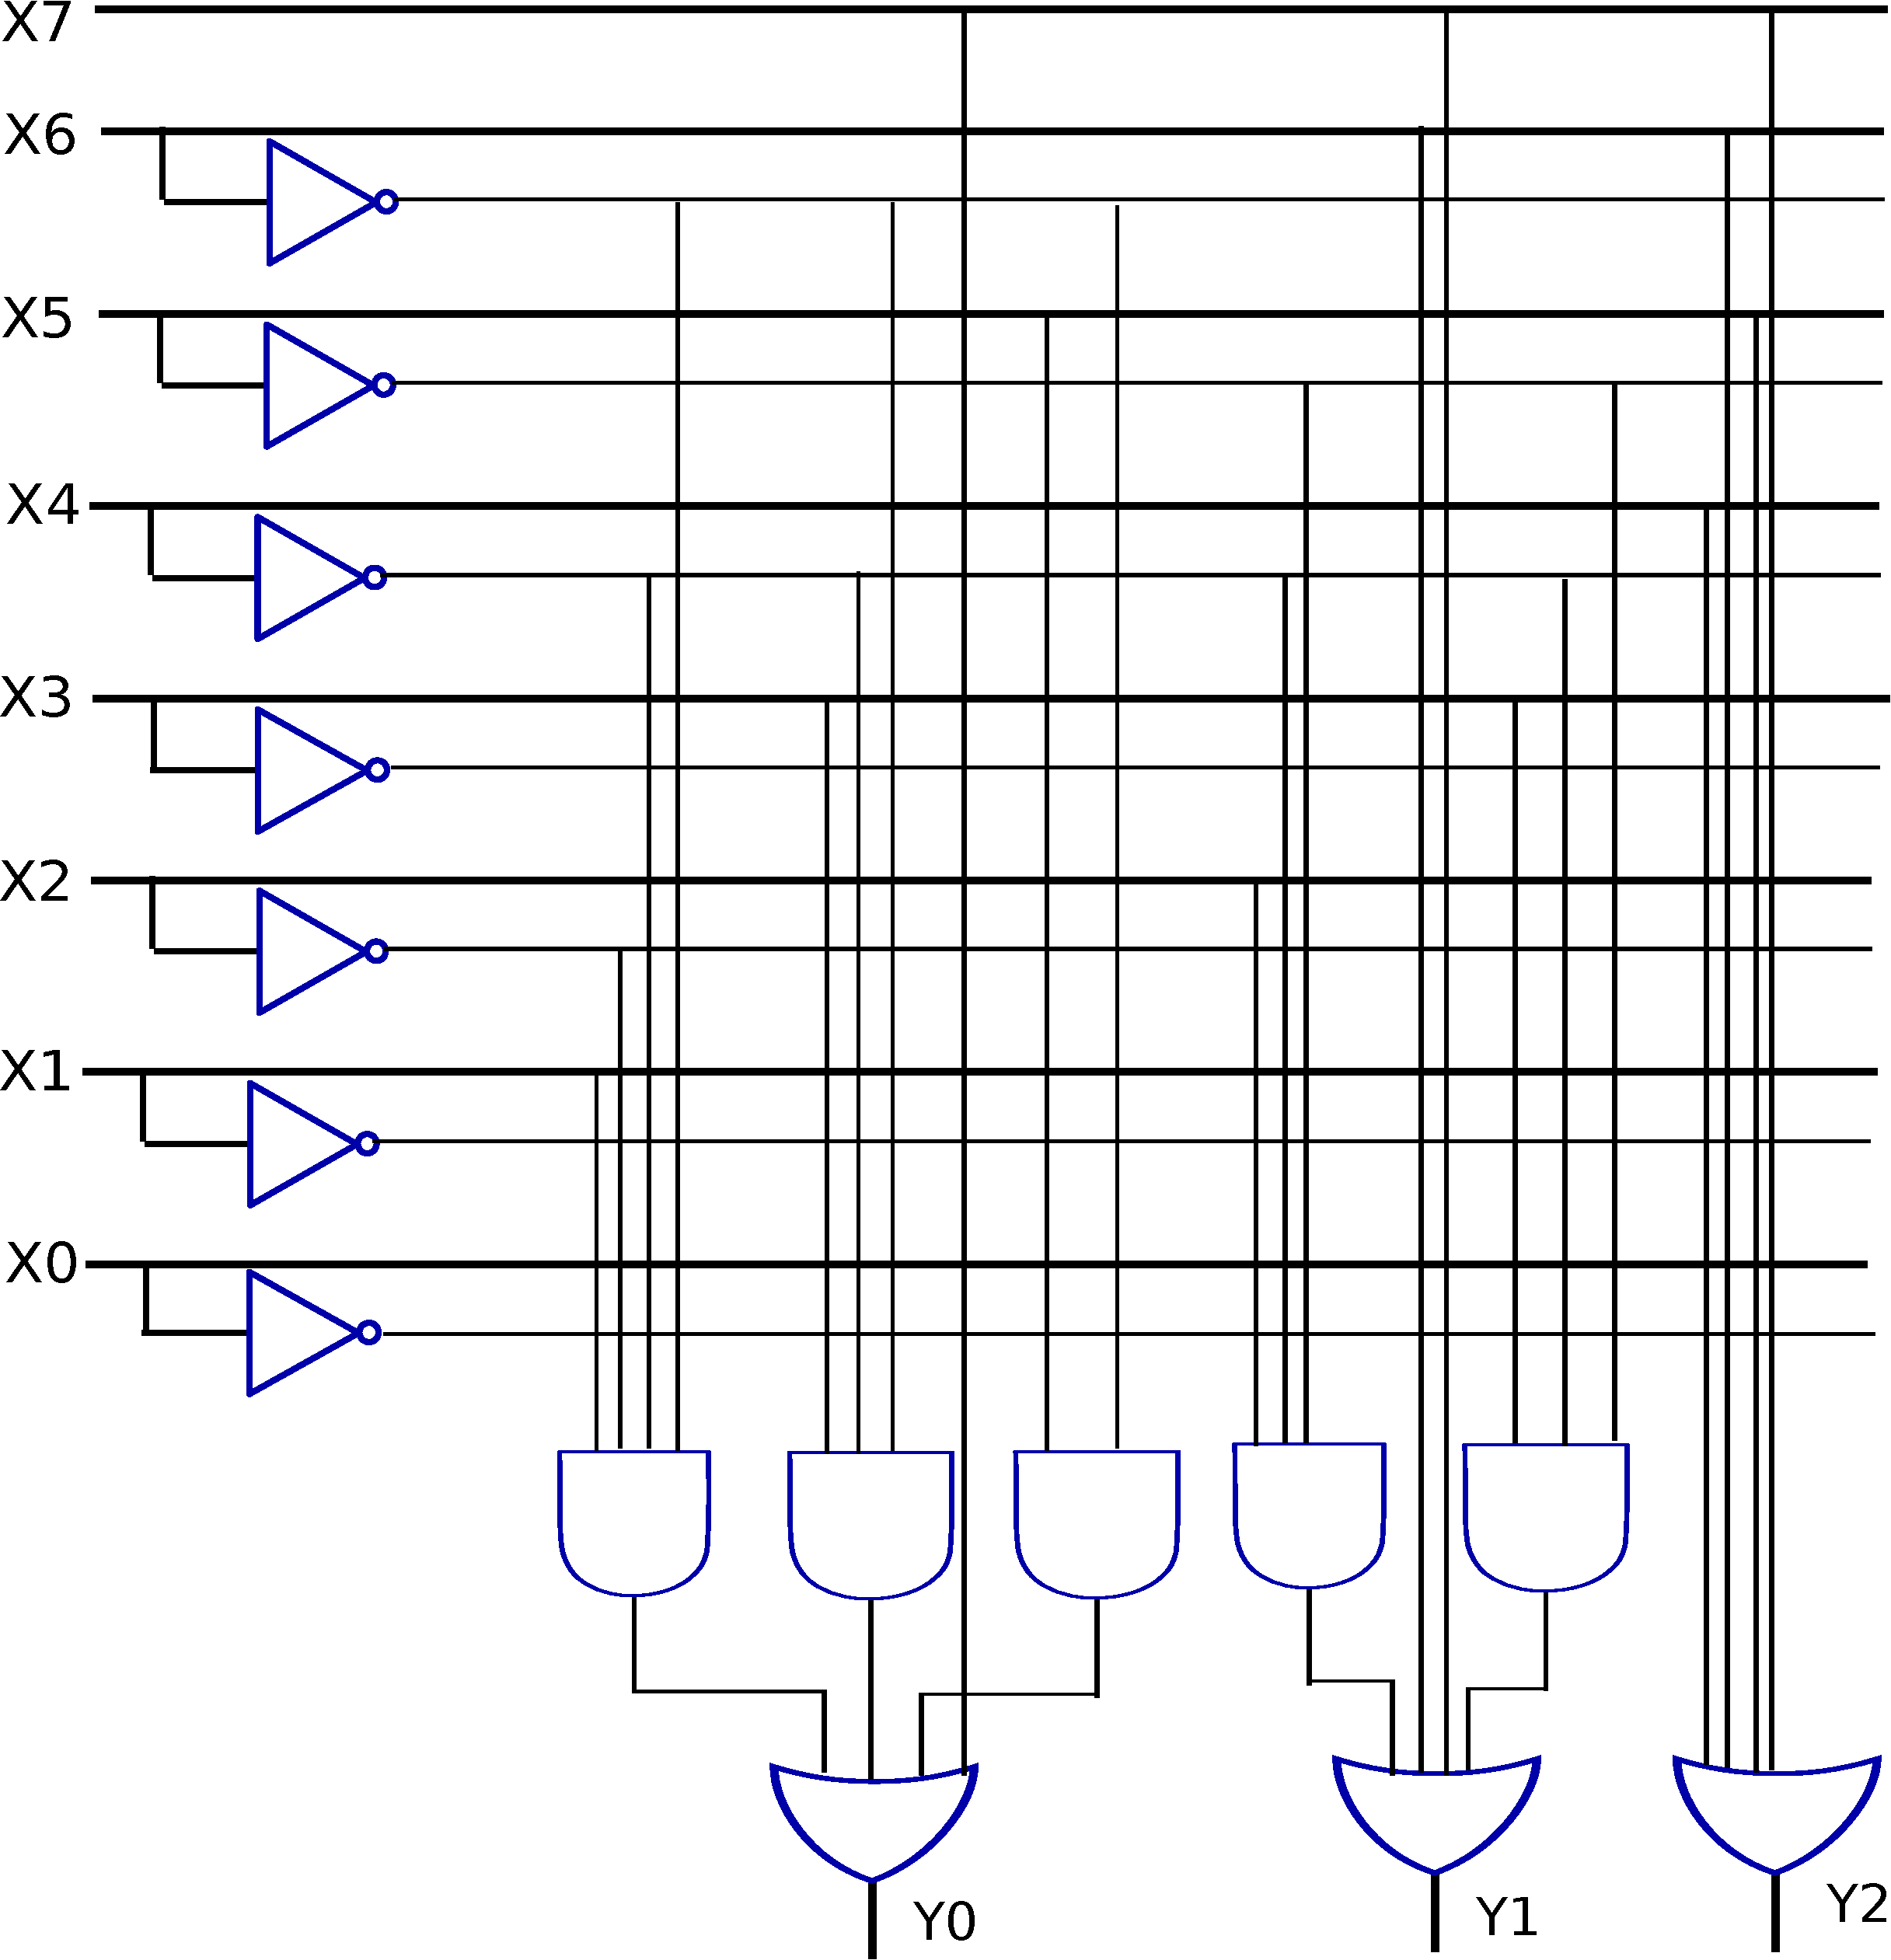
\includegraphics[width=10cm,height=10cm,keepaspectratio]{12.pdf}
\end{figure}

\Exercise
Suppose a poll has to be conducted with three entities A, B and C, each of which can
either vote a `yes' (encoded as 1) or a `no' (encoded as 0). The final output
is equal to the majority opinion. Draw a truth table of the
system, simplify the function, and implement it using logic gates.
\Answer $\newline$

\begin{figure} [H]
  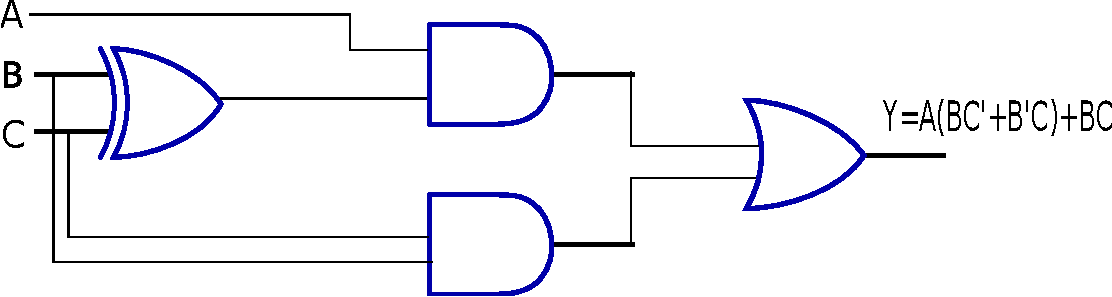
\includegraphics[width=10cm,height=10cm,keepaspectratio]{13.pdf}
\end{figure}



\begin{tabu} to 0.4\textwidth { | X[l] | X[c] | X[cr] |X[r]|}
 \hline
 A & B & C & Y \\
 \hline
 0 & 0 & 0 & 0\\
\hline
 0 & 0 & 1 & 0\\
\hline
 0 & 1 & 0 & 0\\
\hline
 0 & 1 & 1 & 1\\
\hline
 1 & 0 & 0 & 0\\
\hline
 1 & 0 & 1 & 1\\
\hline
 1 & 1 & 0 & 1\\
\hline
 1 & 1 & 1 & 1\\
\hline
\end{tabu}\\

$Y= \overline A BC + A \overline BC + AB\overline C +ABC\newline
 =BC + A(\overline B C+B\overline C) \newline$
 
\Exercise[difficulty=1]
Most circuits in modern computers are built using NAND and NOR gates, because
they are easy to build using CMOS technology.
Suppose another
technology in invented in the near future, 
which implements a new gate, $X$, very efficiently. $X$ takes 3
inputs $A$, $B$ and $C$ and computes:
 $X(A,B,C) = A.B + \overline C$.
Using only X gates and NOT gates, how will you implement the following function:
$f(A,B,C) = A+B+C$?


\Answer
$A+B = X(A,1,\overline B )\\
A+B+C = X(A+B, 1, \overline C )\\
\Rightarrow A+B+C = X(X(A,1,\overline B ),1,\overline C)$

\Exercise[difficulty = 2]
Implement the following logic functions using a 4 to 1 multiplexer, and a single
NOT gate.

\begin{enumerate}[(a) ]
\item
$AB + BC + AC$
\item
$\overline A + \overline B + \overline C$
\item
$A.\overline B + A.B.\overline C$
\end{enumerate}

\Answer 
a)\begin{figure}[H]
  \centering
  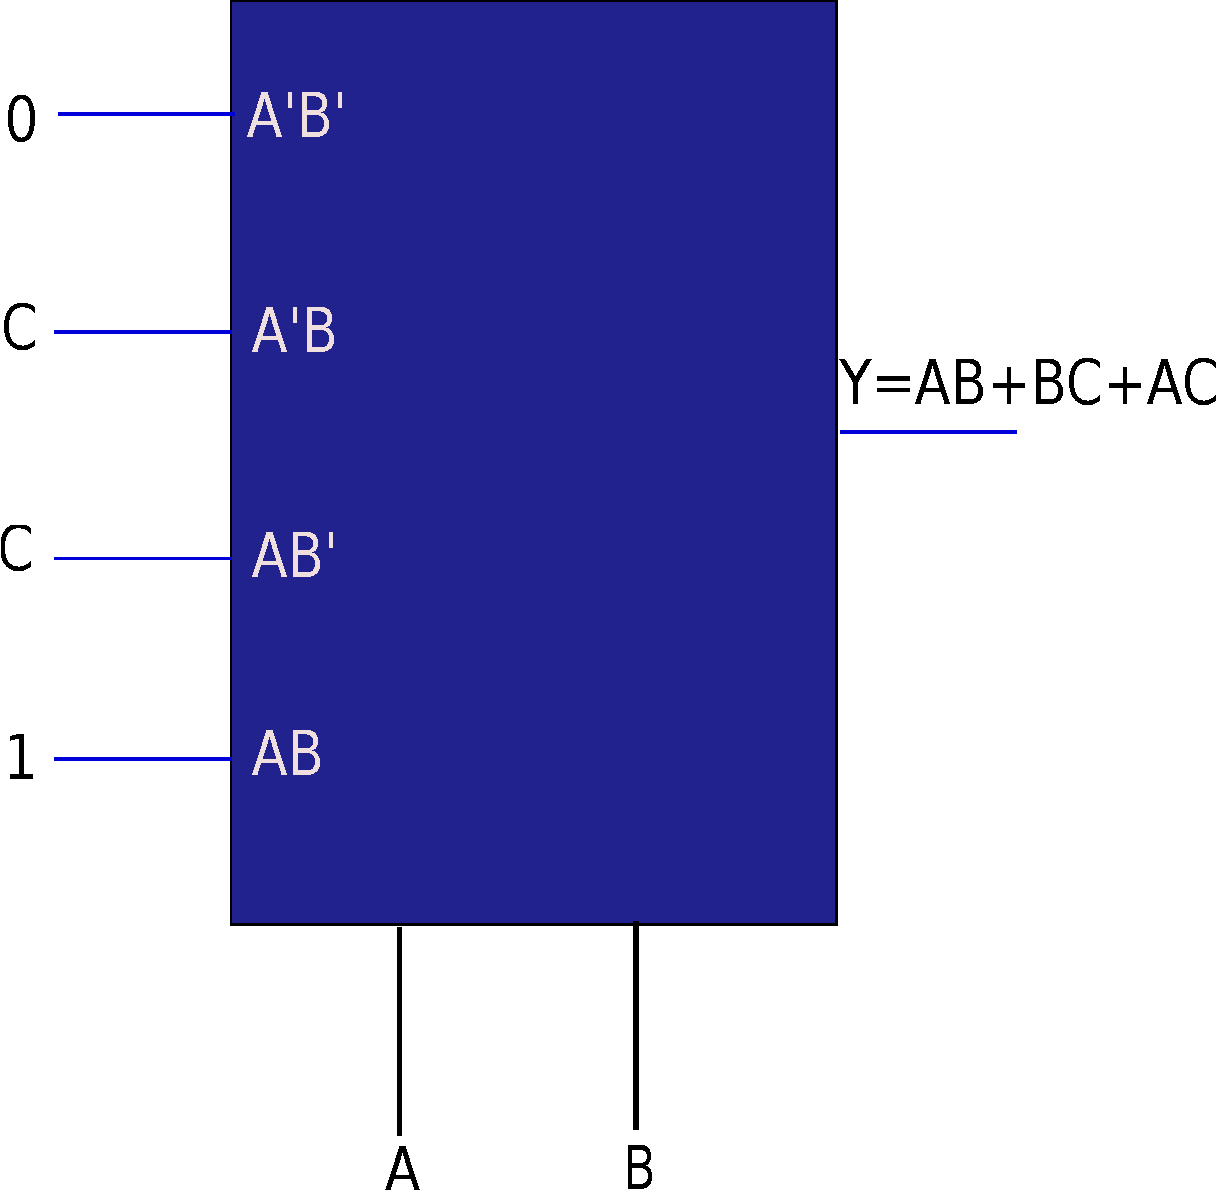
\includegraphics[width=10cm,height=8cm,keepaspectratio]{15a.pdf}
\end{figure}

b)\begin{figure}[H]
  \centering
  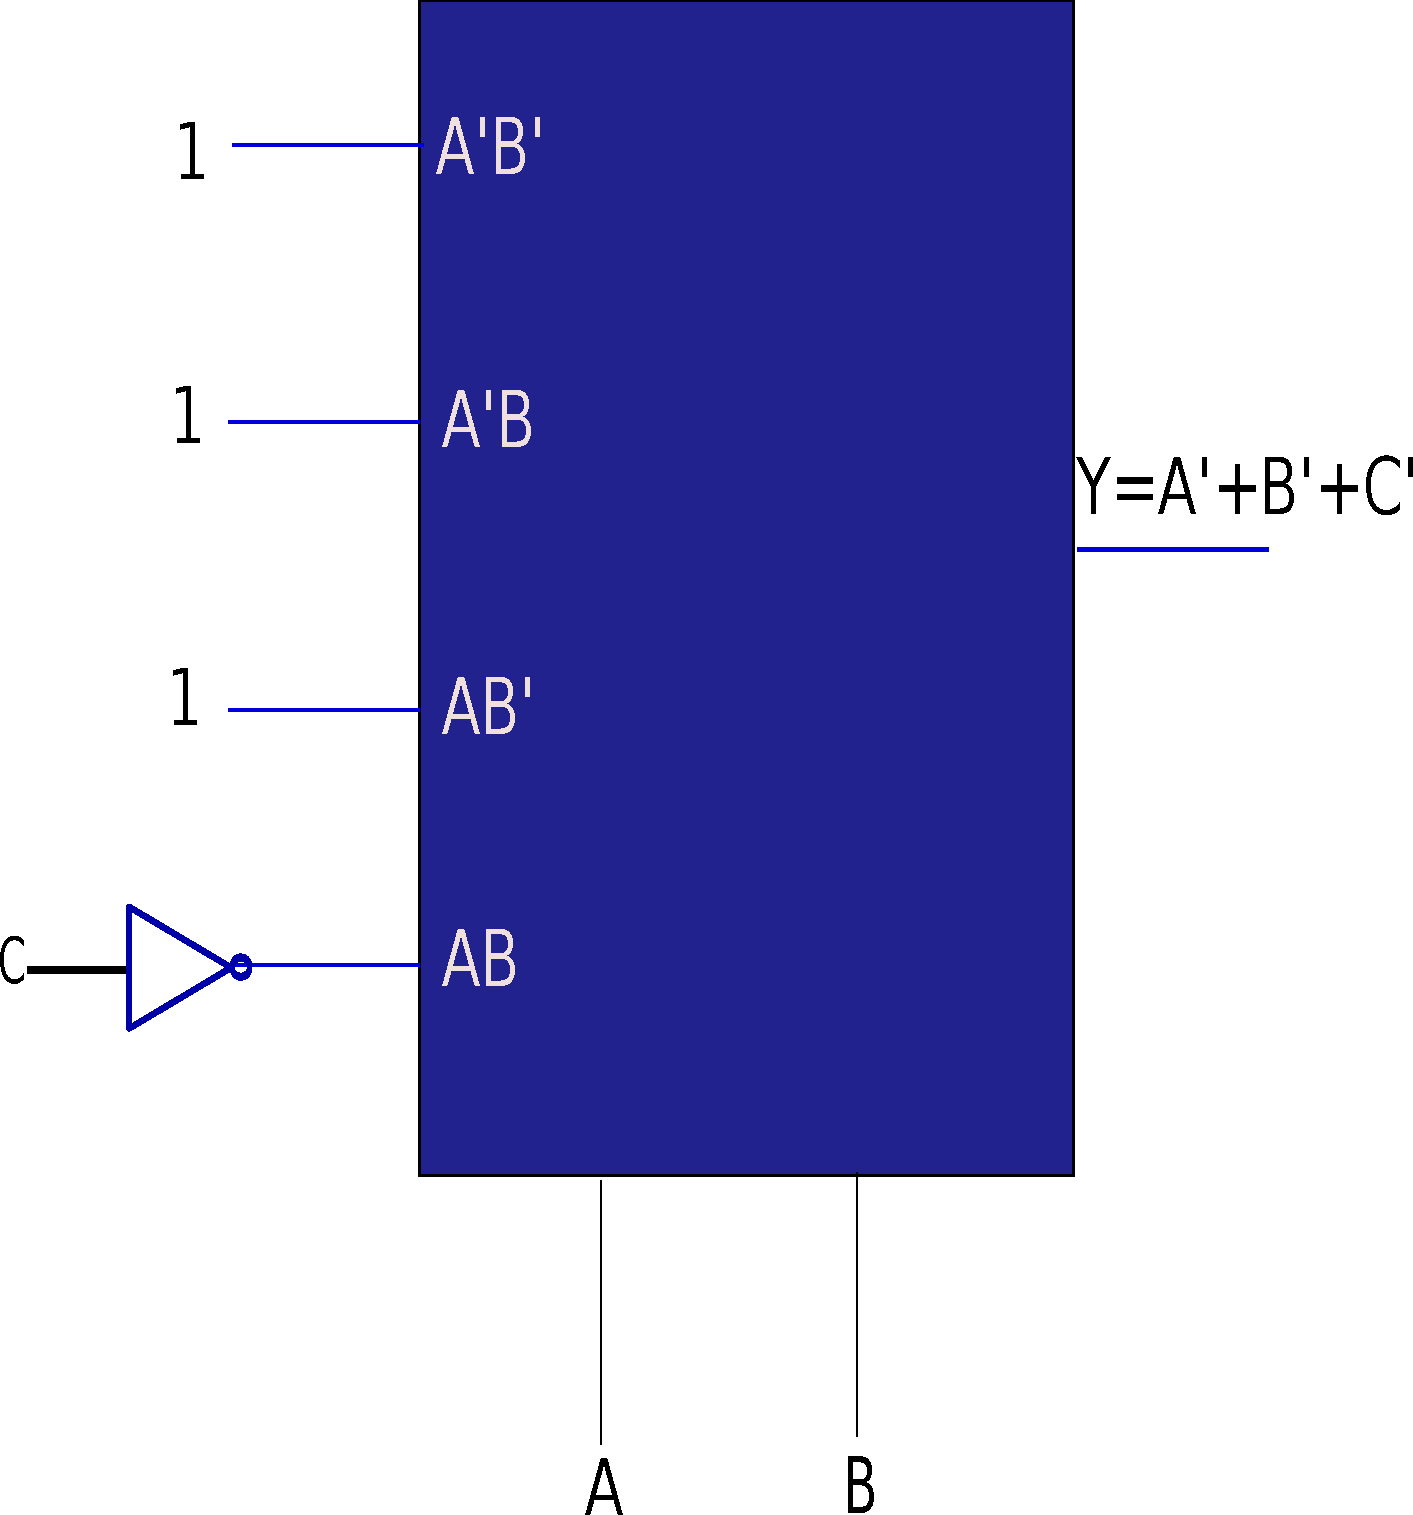
\includegraphics[width=10cm,height=8cm,keepaspectratio]{15b.pdf}
\end{figure}

c)\begin{figure}[H]
  \centering
  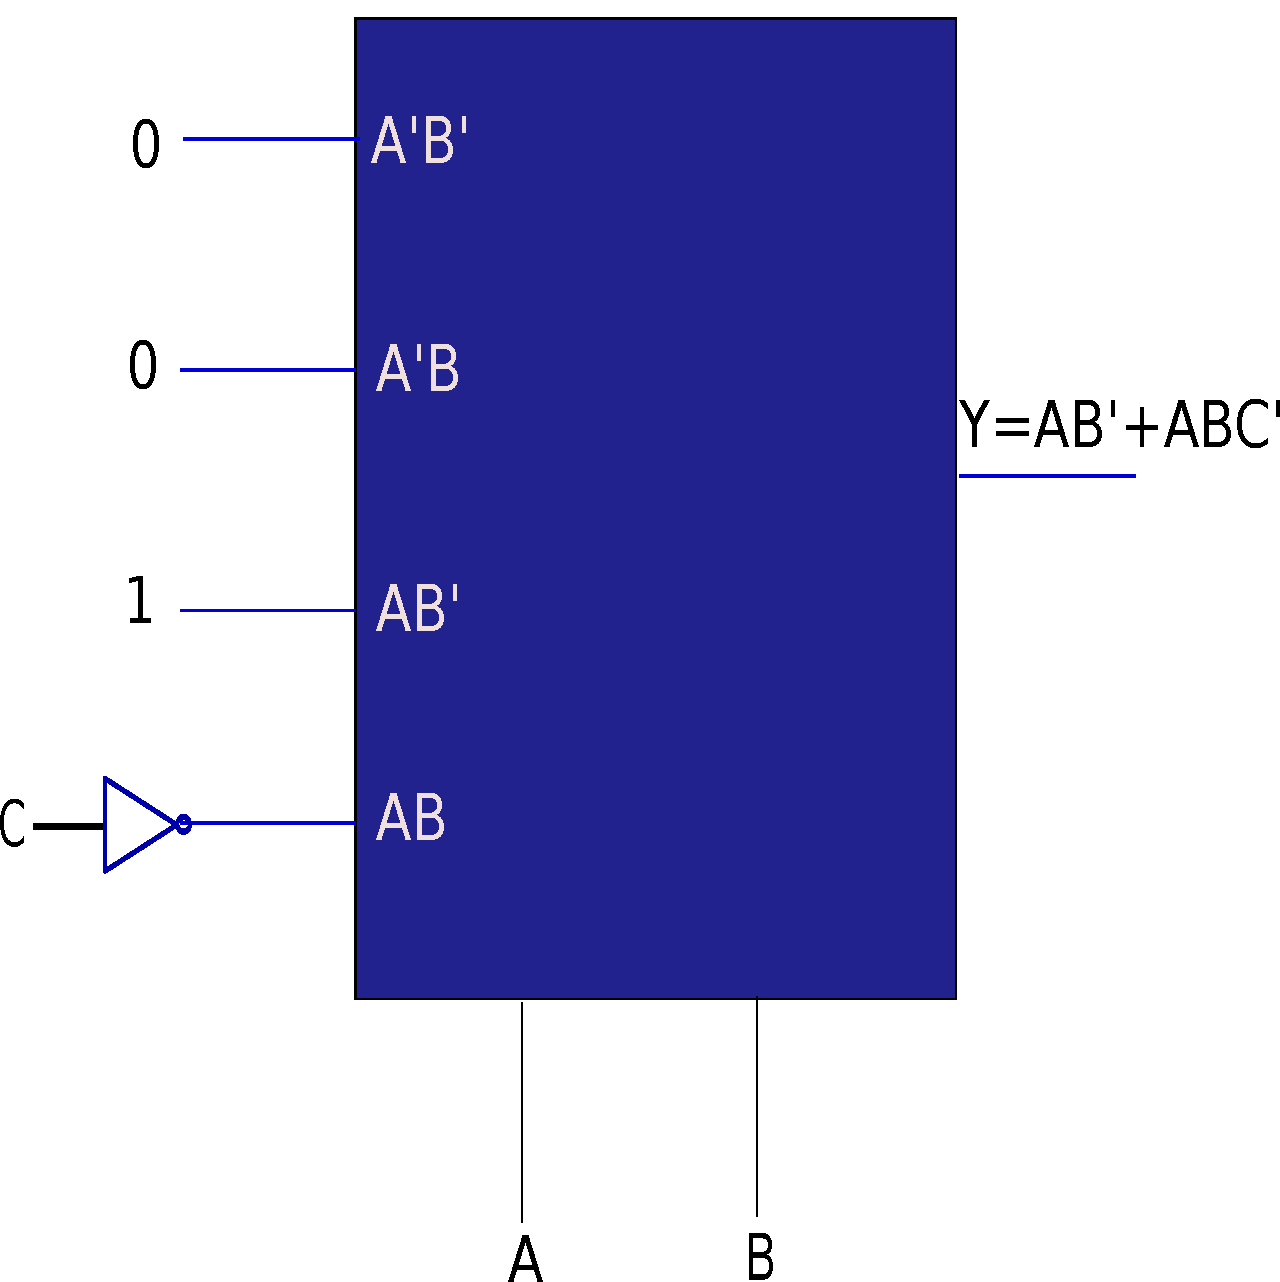
\includegraphics[width=10cm,height=8cm,keepaspectratio]{15c.pdf}
\end{figure}
\Exercise[difficulty=2]
Is it possible to implement every 3 variable Boolean function with a 4 to 1 multiplexer,
and a single NOT gate? Prove your answer.

\Answer
Yes, it is possible.Let $F(A,B,C)$ be the function we want to implement using a $4\times 1$
MUX. The range of this function is \{0, 1\}. We can now define an equivalent
$G(A,B)$ with range \{0, 1, $C$, $\overline C$\} such that for for each given
$A$, $B$ and $C$, $F(A,B,C) = G(A,B)$ . Now giving $A$ and $B$ to the control
lines of the multiplexer, the data lines can be set accordingly , using the truth table to give the correct output. This is possible for every 3 variable Boolean function as every $F(A,B,C)$ can be expressed as $G(A,B)$ which takes only one of the four values - \{0, 1, $C$, $\overline C$\} . Thus, the aforesaid implementation is possible.

\end{ExerciseList}

\section*{Sequential Logic}

\begin{ExerciseList}
\Exercise
What is the difference between a flip-flop and a latch?
\Answer 
1. Latch continuously checks its inputs and changes outputs accordingly. A flip-flop on the other hand, checks its inputs and changes outputs correspondingly, only at times determined by the clocking signal.\\
2. A latch is level-triggered, that is the value of the output is determined at each level of the clock pulse. A flip-flop is edge triggered, that is the output is determined at either the positive/negative edge of the clock pulse. \\
\Exercise
Define the following terms:
\begin{enumerate}[i)]
\item Setup time
\item Hold time
\item Metastability
\item {\em Keep out} region
\end{enumerate}
\Answer 
\hspace{3mm} \\
a) \textit{Setup time}: The units of time for which the input is desired to be kept stable before the triggering of the clock pulse is called \textit{setup time}. \\
b) \textit{Hold time}: The units of time for which the input is desired to be kept stable after the triggering of the clock pulse is called \textit{hold time}. \\
c) \textit{Metastability}: The phenomenon in which the output of a flip-flop becomes non-deterministic, fluctuating and oscillating due to a change in the input during positive/negative edge of the clock, depending on the type of edge-triggering, is called \textit{metastability}. \\
d) \textit{Keep-out region}: The window of time during which it is desired to keep the inputs stable is called \textit{keep-out region}. \\
\Exercise
Why do we wish to avoid the indeterminate state in an S-R flip-flop?
\Answer
The SR flip-flop using NAND gates gives an indeterminate output when both S and R are equal to 1. We need to avoid this as it may result in a race condition, and the output can become unpredictable. The output keeps oscillating/fluctuating between 0 and 1. 
\Exercise
What is the advantage of an edge sensitive flip-flop?
\Answer
In a level sensitive flipflop, circuits have half a clock cycle to compute the correct outputs ie: when the clock is 0. When the clock is 1 (high), the outputs are visible. In an edge sensitive flip-flop, changes are visible only at the upward/downward edge of a clock. This gives us more accurate results since a unique well-defined point is needed for determination of accurate outputs. Also, an edge sensitive flip-flop gives one full cycle for computation of correct outputs. Another issue is with the circuits that have feedback (the outputs are connected back to the inputs) where level triggering causes chaos, because the level is wide enough (half a clock cycle) that the output can feed back to the inputs within the same period, and output becomes unpredictable.     \\
\Exercise[difficulty = 1]
What is the fundamental advantage of a JK flip-flop over a D flip-flop? 
\Answer
The fundamental advantage is that a JK flip-flop is used for toggling by shorting the inputs J and K and giving it a logical 1. The D flipflop has only (J=1 and K=0 and viceversa) states when enabled, and latches the previous state values when disabled. Thus, a JK flip-flop can be used like a D flip-flop with toggling.
 
\Exercise
Describe the design of registers in your own words.
\Answer
Registers are groups of flip-flops, where each flip-flop is capable of storing one bit of information. An $n$-bit register is a group of n flip-flops. The basic function of a register is to hold information in a digital system and make it available to the logic elements for the computing process. Registers consist of a finite number of flip-flops. Since each flip-flop is capable of storing either a "0" or a "1", there is a finite number of 0-1 combinations that can be stored into a register. Each of those combinations is known as state or content of the register. There are many types of registers: \\
1. \textit{Parallel-in Parallel out}: \\
This can be designed using D flipflops where each D flipflop is connected to an input line. The $n$ bits are loaded in parallel to each of the $n$ D flipflops and are also read out in parallel at every negative or positive clock edge. \\
2. \textit{Serial-in Parallel out}: \\
This can be designed using D flipflops, where we have a single input that is fed to the leftmost D flip-flop. Every cycle, the input moves to the adjacent flip-flop on the right. Thus, in order to load $n$ bits, it takes $n$ cycles. The first bit will get loaded into the leftmost flipflop in the first cycle, and it will take $n$ cycles for it to reach the last flipflop. Then, the output is taken by reading all the $n$ bits in parallel. This is also known as \textit{shift} register. \\

\Exercise
An edge sensitive toggle flip-flop (or T flip-flop) is the one which takes a
clock signal and a single input T and toggles its output on every rising (or
falling) clock edge. How will you construct an edge sensitive T flip-flop form
an edge sensitive J-K flip-flop?

\Answer
Short the inputs J and K of J-K flip-flop into a single wire and call it T.
When T=1 (i.e. J=1 and K=1) the output toggles every clock edge (of same
direction), and when T=0 (i.e. J=0 and K=0), the output remains same.

\Exercise[difficulty=1]
Can you create a negative edge triggered D flipflop using two 2 multiplexers, and a NOT gate?
\begin{figure}[H]
  \centering
  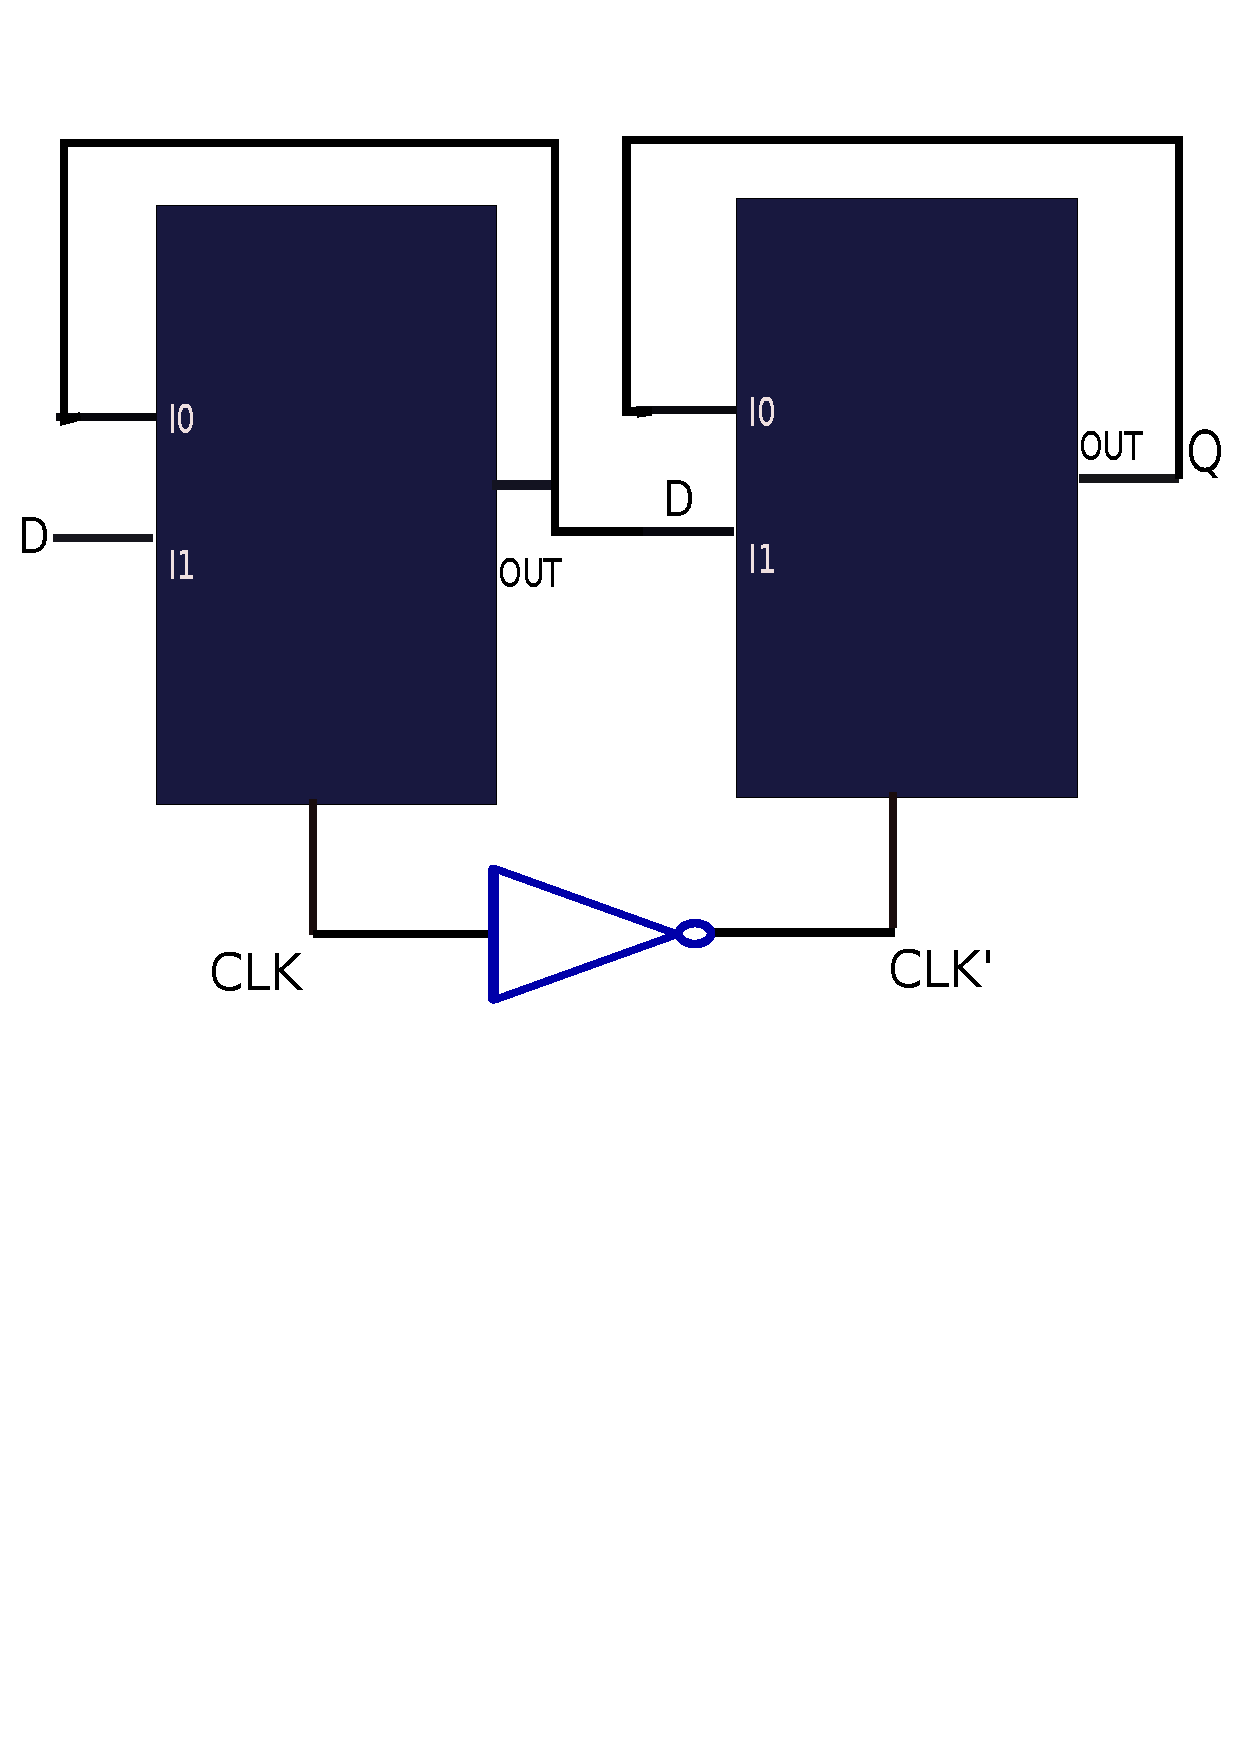
\includegraphics[width=10cm,height=8cm,keepaspectratio]{24.pdf}
  \caption{}
\end{figure}
\Exercise
Design a SR flip-flop with NOR gates.
\begin{figure}[H]
  \centering
  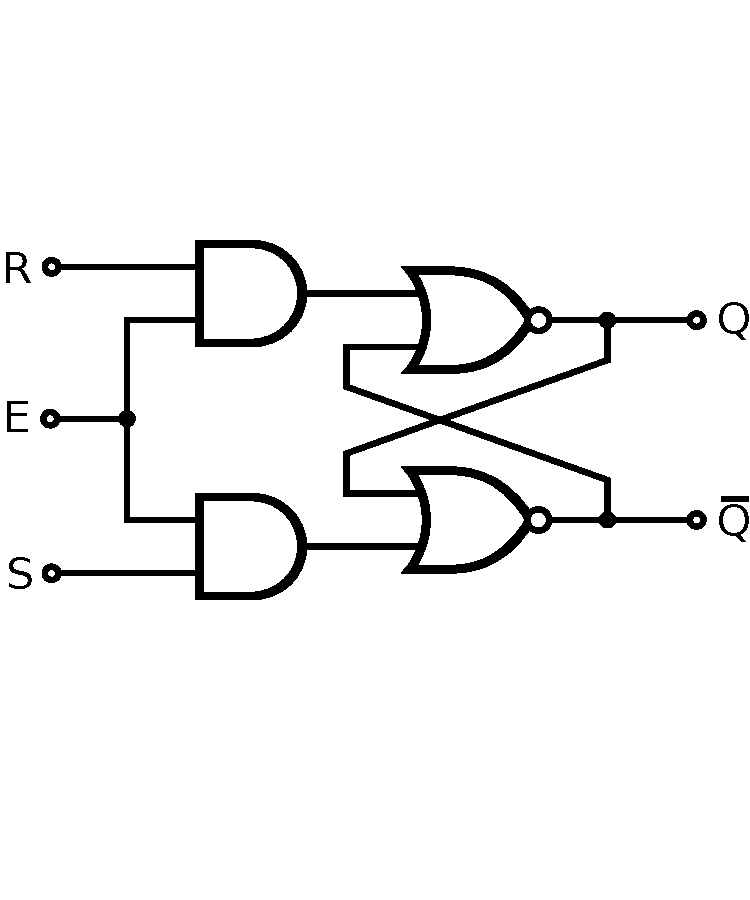
\includegraphics[width=10cm,height=4cm,keepaspectratio]{25.pdf}
\end{figure}
\Exercise
Using only two edge triggered D flip-flops design a circuit, which divides
the frequency of an input signal (clock) by 4. 
\begin{figure}[H]
  \centering
  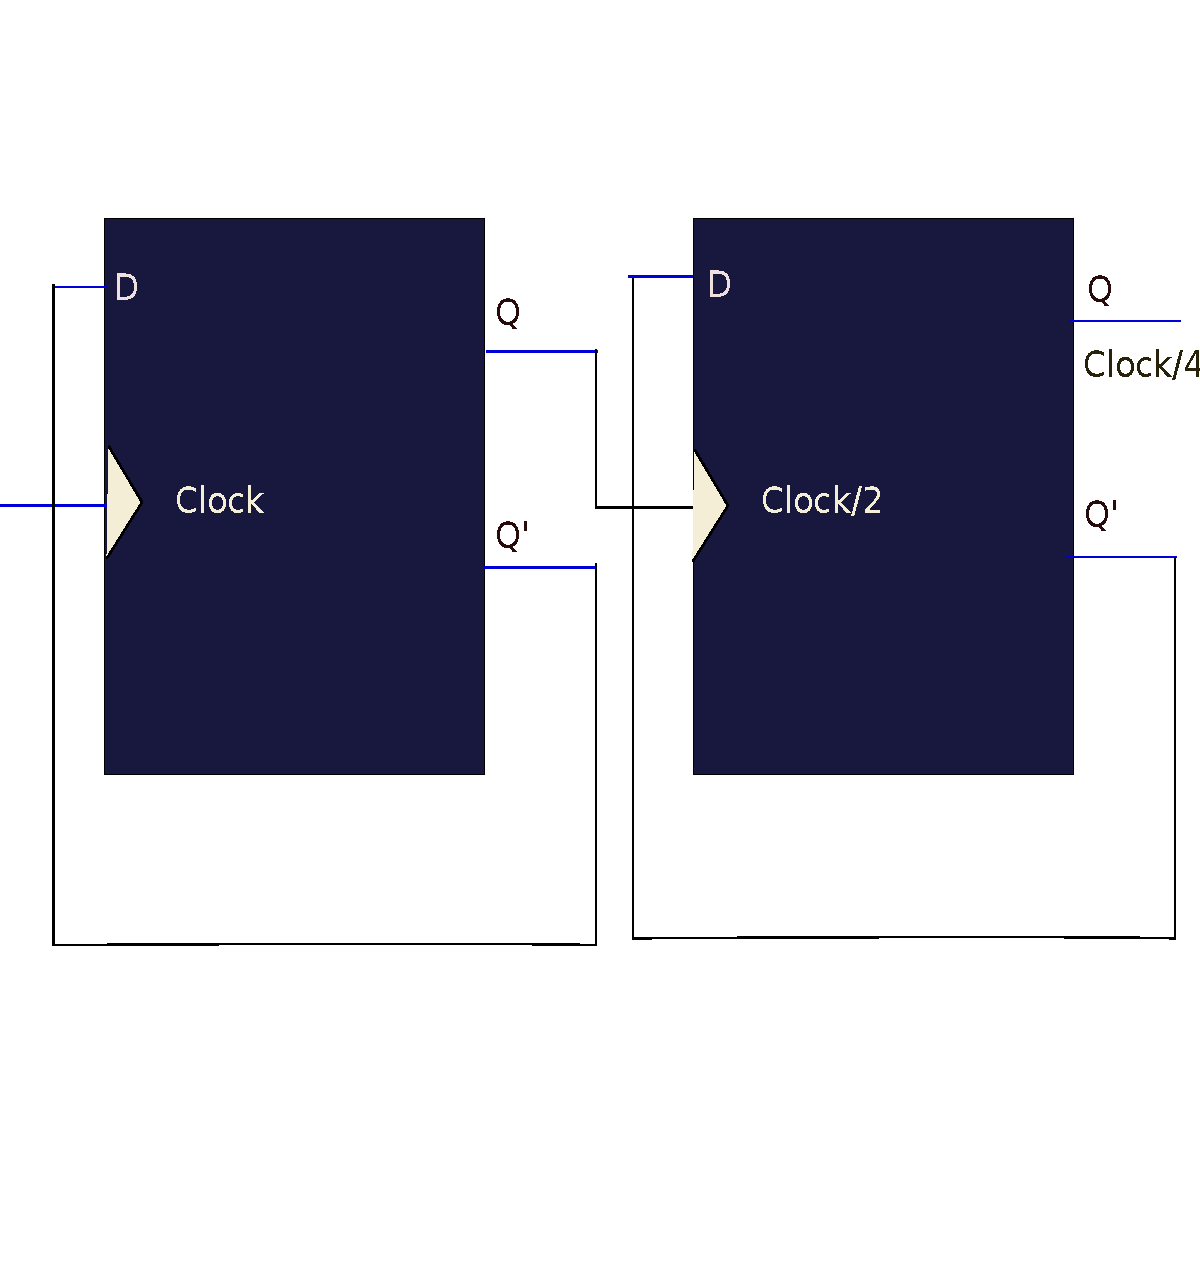
\includegraphics[width=10cm,height=8cm,keepaspectratio]{26.pdf}
  \caption{}
\end{figure}

\Exercise[difficulty=2]
Counters are essential components of any complex digital circuit. They are
essentially sequential circuits which loop through a specific set of states.
Design
a counter which generates 
a sequence of numbers (in binary form) from 0 to 7 and cycles back again to 0.
This is called a MOD 8 counter. 

\Answer
Any logic circuit with $n$ states can be made with at most $(\lceil \log_2 n \rceil)$ D flip-flops. So this circuit can be made using 
3 D flip-flops.\\

Let $D0$, $D1$, $D2$ and $Q0$, $Q1$, $Q2$ be the corresponding inputs and outputs of the 3 flip-flops.
$Qi_{now}$ is the present value of $Qi$ and $Qi_{next}$ is the next value of $Qi$ which is obtained by shorting $Qi_{now}$ with $Qi$ and  $Qi_{next}$ and $Di$. 
State table for the circuit:\\

\begin{tabular}{|c|c|c|c|c|c|}
\hline
$Q0_{now}$ & $Q1_{now}$ & $Q2_{now}$ & $Q0_{next}$ & $Q1_{next}$ & $Q2_{next}$ \\
\hline
0 & 0 & 0 & 0 & 0 & 1\\ 
\hline
0 & 0 & 1 & 0 & 1 & 0\\
\hline
0 & 1 & 0 & 0 & 1 & 1\\
\hline
0 & 1 & 1 & 1 & 0 & 0\\
\hline
1 & 0 & 0 & 1 & 0 & 1\\
\hline
1 & 0 & 1 & 1 & 1 & 0\\
\hline
1 & 1 & 0 & 1 & 1 & 1\\
\hline
1 & 1 & 1 & 0 & 0 & 0\\
\hline
\end{tabular} \\


Using K-maps, we simplify the logic function to obtain $Q_{next}$ (or $D$) in terms of $Q_{now}$ (or $Q$).\\
\\
$D0 = \overline {Q0}.Q1.Q2 + Q0.\overline{Q1}+Q0.\overline{Q2}\\
D1 = \overline{Q1}.Q2 + Q1.\overline{Q2}\\
D2 = \overline{Q2}$ \\
\\
This circuit can be implemented using simple logic gates. The output states are given by $Q0$ (MSB), $Q1$ and $Q2$ (LSB).
\Exercise[difficulty=2]
Using D flip-flops and logic gates, design a circuit, which generates the following sequence of numbers:
\[
001 \rightarrow 100 \rightarrow 010 \rightarrow 101 \rightarrow 110
\rightarrow 111 \rightarrow 011 \rightarrow 001 
\]

Assume that the circuit
never generates 000. This circuit can be used to generate pseudo-random numbers.

\Answer:
State table for the circuit:\\

\begin{tabular}{|c|c|c|c|c|c|}
\hline
$Q0$ & $Q1$ & $Q2$ & $D0$ & $D1$ & $D2$ \\
\hline
0 & 0 & 1 & 1 & 0 & 0\\ 
\hline
1 & 0 & 0 & 0 & 1 & 0\\
\hline
0 & 1 & 0 & 1 & 0 & 1\\
\hline
1 & 0 & 1 & 1 & 1 & 0\\
\hline
1 & 1 & 0 & 1 & 1 & 1\\
\hline
1 & 1 & 1 & 0 & 1 & 1\\
\hline
0 & 1 & 1 & 0 & 0 & 1\\
\hline
\end{tabular} \\

Here, \\
$D0 = Q1 \oplus Q2\\
D1 = Q0\\
D2 = Q1$\\


\end{ExerciseList}

\section*{Memories}

\begin{ExerciseList}

\Exercise
Compare the power, area and time of a SRAM, DRAM, and latch.

\Answer:\\
\begin{tabular}{||l|p{3cm}|p{3cm}|p{3cm}||}
\hline
\hline
 & Power & Area & Time per Access \\
\hline
SRAM & Medium  & Medium  &  Medium\\
\hline
DRAM & Low & Low & High \\
\hline
Latch & High & High & Low \\
\hline
\hline
\end{tabular}

\Exercise
Propose a design for the column mux/demux circuit.

\Exercise
What is the role of the {\em match} line in a CAM array?
\Answer
The {\em match} line is used to check if there is a match between the value stored in the CAM array and the input bit. A CAM array is addressed by its content, and we need to index each row by its content and be able to find out if there is a match between the content of the CAM cells and the input address bits or not. Hence, the {\em match} line is required. \\
Let V be the value stored in the CAM cell, and $A_i$ be the value of the input bit. If V=$\overline A_i$ , then by the transistor logic, the match line will be pulled to a logical 0 by one pair of the pass transistors. This indicates a mismatch between the input bit and the content of the CAM cell. However, if V= $A_i$, then the match line will be equal to a logical 1, indicating a match. \\
We can compare each row of the CAM cell with the input, A. If any row matches the input, the corresponding match line will have a value of 1. We can compute a logical OR of all the match lines, and decide if we can have a match in a CAM array or not. Also, all the match lines of the CAM array could be connected to a priority encoder to find the index of the row that matches the data. \\
\Exercise
What is the role of the {\em refresh logic} in a DRAM array?
\Answer
Suppose the capacitor in a DRAM cell is charged to a voltage equal to the supply voltage. In practice, the capacitor will gradually leak some charge though the dielectric, and the transistor. This current, though small, can be significant for a longer duration due to loss of charge, and ultimately discharge the capacitor. To prevent this, we need a {\em refresh logic}, or {\em refresh circuitry} to periodically refresh the value of a DRAM cell. We need to read the value and write it back. This needs to be done after a read operation as well because the capacitor loses some charge while charging the bit line. \\ 
\Exercise
Describe the design of a ROM and PROM cell.
\Answer
1. \textit{ROM cell} : \\
The structure of a ROM cell is similar to that of a DRAM cell. The capacitor in a DRAM cell stores a logical bit. If it stores a logical 1, then the charge across the capacitor is equal to the supply voltage $V_{dd}$, and if it stores a logical 0, then the charge across the capacitor is 0 V. Instead of having a capacitor, we can directly connect one end of the transistor to either ground or $V_{dd}$ depending on the bit that we wish to store. This is done at the time of manufacturing a chip. Hence, a ROM cell replaces the capacitor by a direct connection to $V_{dd}$ or ground. \\ \\
2. \textit{PROM cell} : \\
A PROM cell can be programmed once to store either a logical 1 or 0. Here, the connection between the transistor and ground is through an element called \textit{antifuse}. It is a weak conductor. When we transfer a large amount of current through the antifuse, it forms a conducting path, and drives the bit line to a logical 0. In this case, the cell stores a logical 0. Normally, when it does not form any conducting path, it does not have the ability to drive the bit line to a logical 0, and hence we infer that the cell stores a logical 1. Each bit line is precharged. After enabling the word line, if the voltage at the sense amplifiers does not increase then we can infer a logical 1. However, if the voltage keeps decreasing towards 0 V, then we can infer a logical 0. \\ 
\Exercise
Design a single PLA array to compute al the following Boolean functions:

\begin{enumerate}[a)]
\item  $A.B + B.C + C.A$
\item  $A.\overline{B}.\overline{C} + \overline{A}.B.C$
\item  $\overline{A+B}$
\end{enumerate}
\Answer
\begin{figure}[H]
  \centering
  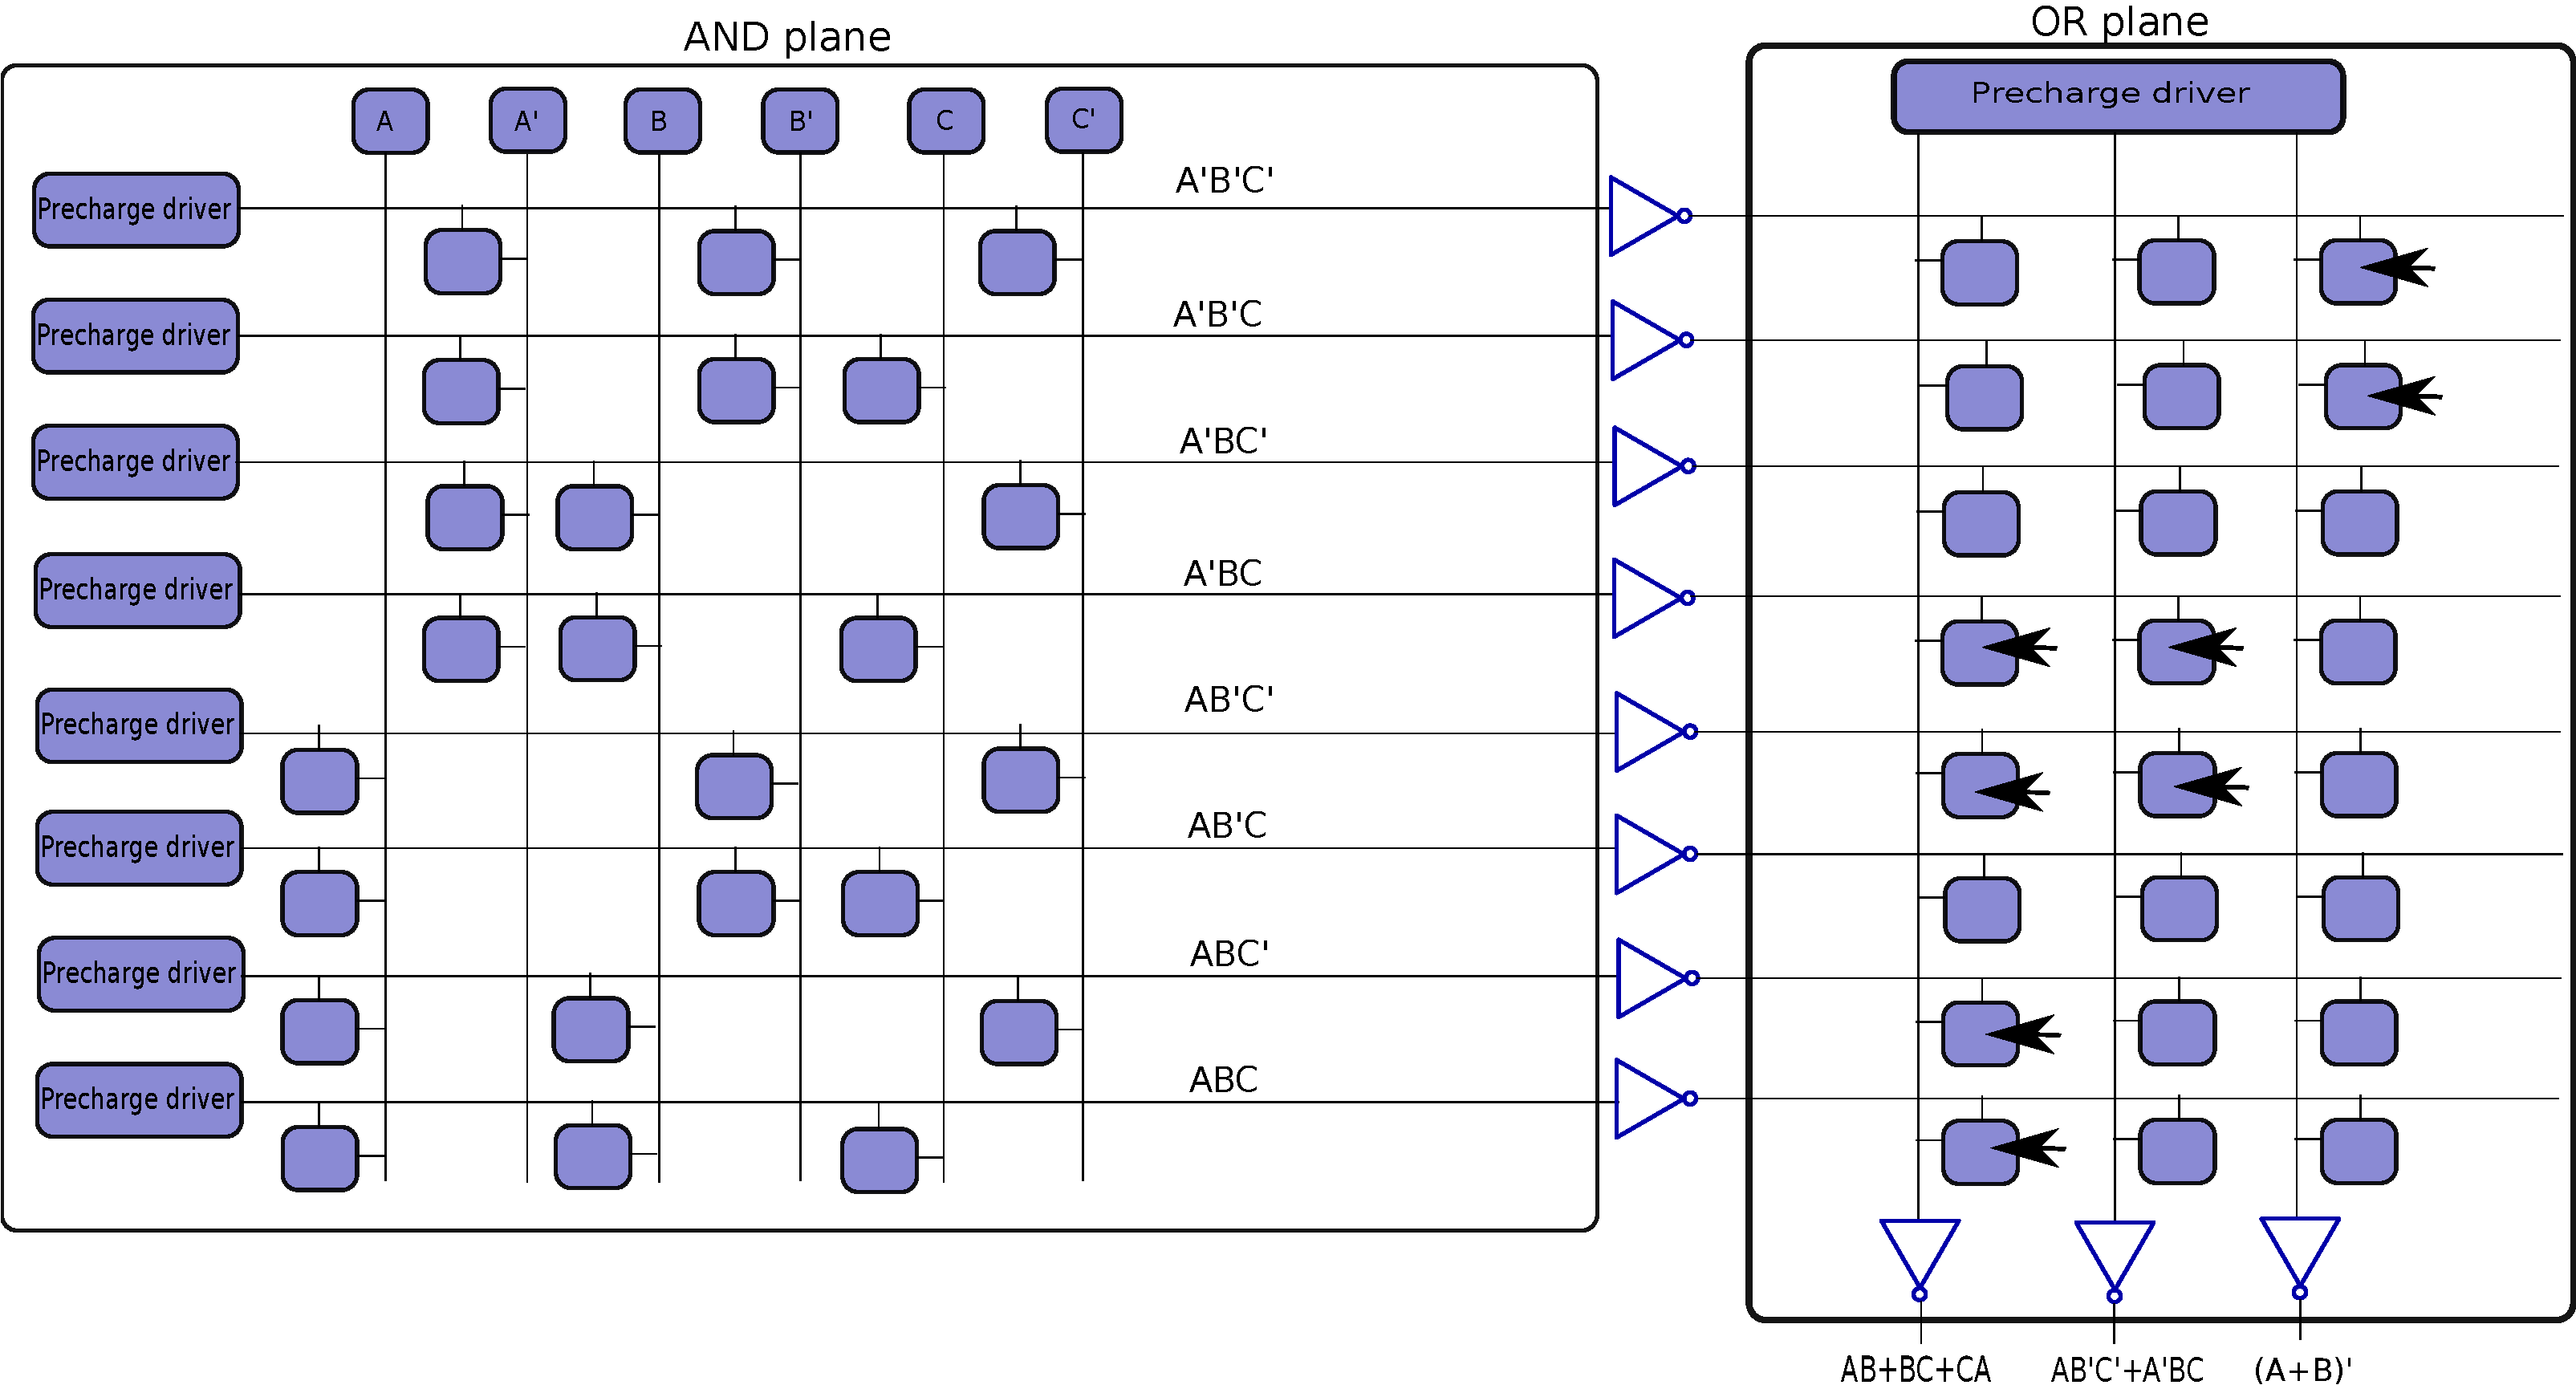
\includegraphics[width=17cm,height=30cm,keepaspectratio]{PLA.pdf}
  \caption{}
\end{figure}
\end{ExerciseList}

\section*{Design Problems}

\begin{ExerciseList}
\Exercise
Design the following circuits using a circuit simulator such as Spice and verify their operation:

\begin{enumerate}[a)]
\item NOT gate
\item NAND gate
\item D flip-flop
\item SRAM cell
\end{enumerate}

\Exercise
Prepare a report on novel memory technologies such as phase change memory, Ferro-electric
RAM, and magneto-resistive RAM. 
\end{ExerciseList}
